\documentclass[a4paper,12pt]{article}

\documentclass[a4paper,12pt]{article}
	
\usepackage[T2A]{fontenc}			
\usepackage[utf8]{inputenc}			
\usepackage[english,russian]{babel}	

\usepackage[
bookmarks=true, colorlinks=true, unicode=true,
urlcolor=black,linkcolor=black, anchorcolor=black,
citecolor=black, menucolor=black, filecolor=black,
]{hyperref}

\usepackage{color}
\usepackage{caption}


\usepackage{amsmath,amsfonts,amssymb,amsthm,mathtools} 
\usepackage{wasysym}

\usepackage{graphicx}
%\usepackage[cache=false]{minted}
\usepackage{cmap}
\usepackage{indentfirst}

\usepackage{listings} 
\usepackage{fancyvrb}
\usepackage{slashbox}

\usepackage{geometry}
\geometry{left=2cm}
\geometry{right=1.5cm}
\geometry{top=1cm}
\geometry{bottom=2cm}

\setlength{\parindent}{5ex}
\setlength{\parskip}{0.5em}

\usepackage{titlesec}
\usepackage{pgfplots}
\usepackage{filecontents}
\usetikzlibrary{datavisualization}
\usetikzlibrary{datavisualization.formats.functions}

\DeclareCaptionFont{white}{\color{white}}
\DeclareCaptionFormat{listing}{\colorbox{gray}{\parbox{\textwidth}{#1#2#3}}}
\captionsetup[lstlisting]{format=listing,labelfont=white,textfont=white}
\lstloadlanguages{% Check Dokumentation for further languages ...
C,
C++,
csh,
Java
}

\definecolor{red}{rgb}{0.6,0,0} % for strings
\definecolor{blue}{rgb}{0,0,0.6}
\definecolor{green}{rgb}{0,0.8,0}
\definecolor{cyan}{rgb}{0.0,0.6,0.6}

\lstset{ %
language=Lisp,                 % выбор языка для подсветки
basicstyle=\small\sffamily, % размер и начертание шрифта для подсветки кода
numbers=left,               % где поставить нумерацию строк (слева\справа)
numberstyle=\tiny,           % размер шрифта для номеров строк
stepnumber=1,                   % размер шага между двумя номерами строк
numbersep=5pt,                % как далеко отстоят номера строк от подсвечиваемого кода
showspaces=false,
backgroundcolor=\color{white},         
showstringspaces=false,      % показывать или нет пробелы в строках
showtabs=false,             % показывать или нет табуляцию в строках
frame=single,              % рисовать рамку вокруг кода
tabsize=2,                 % размер табуляции по умолчанию равен 2 пробелам
captionpos=t,              % позиция заголовка вверху [t] или внизу [b] 
breaklines=true,           % автоматически переносить строки (да\нет)
breakatwhitespace=false, % переносить строки только если есть пробел
escapeinside={\%*}{*)}
}

% Для измененных титулов глав:
\definecolor{gray75}{gray}{0.75} % определяем цвет
\newcommand{\hsp}{\hspace{20pt}} % длина линии в 20pt
% titleformat определяет стиль
\titleformat{\chapter}[hang]{\Huge\bfseries}{\thechapter\hsp\textcolor{gray75}{|}\hsp}{0pt}{\Huge\bfseries}

\begin{document}
	
	\begin{figure}[h!]
	\begin{center}
		{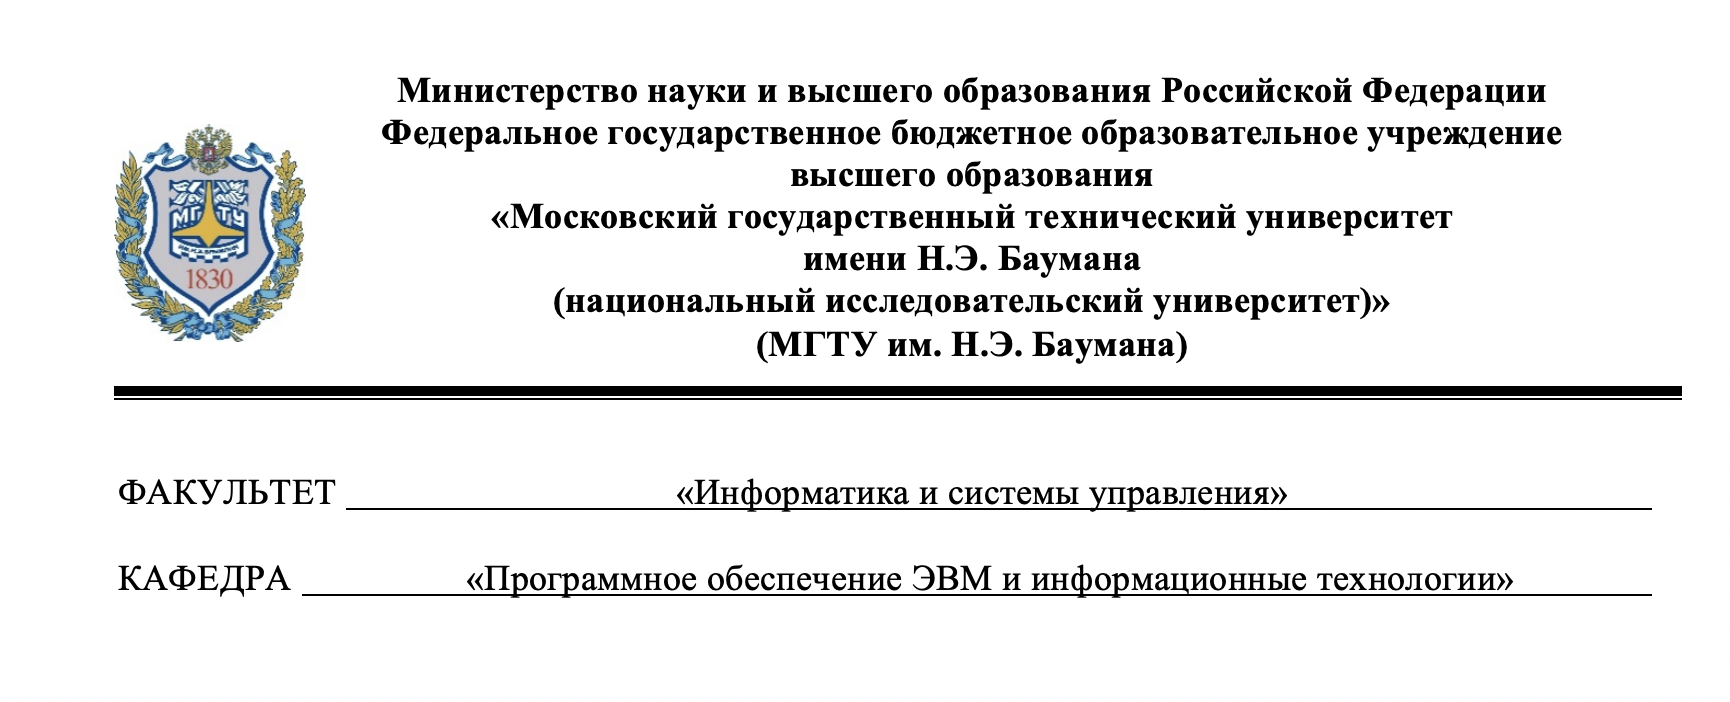
\includegraphics[width = \textwidth]{titul.png}}
	\end{center}
\end{figure}

\vspace*{20mm}

\huge
\begin{center}
	Лабораторная работа №10\\
	Рекурсивные функции
\end{center}


\vspace*{45mm}

\large
\begin{flushleft}
	Студент: Луговой Д.М. \\
	Группа: ИУ7-61Б \\
	Преподаватель: Толпинская Н.Б.
\end{flushleft}

\vspace*{55mm}

\large
\begin{center}
	Москва, 2020 г.
\end{center}

\thispagestyle{empty}
	
	\textbf{Цель работы}: получить навыки построения модели предметной области, разработки и оформления программы на Prolog, изучить принципы, логику формирования программы и отдельные шаги выполнения программы на Prolog.\\
	
	\textbf{Задачи работы}: приобрести навыки декларативного описания предметной области с использованием фактов и правил.
	Изучить способы использования термов, переменных, фактов и правил в программе на Prolog, принципы  и правила сопоставления и отождествления, порядок унификации.
	
\section*{Задание}
	
Используя  базу знаний, хранящую знания (лаб. 13):
\begin{itemize}
	\item «Телефонный справочник»: Фамилия, №тел, Адрес – структура (Город, Улица, №дома, №кв),
	\item «Автомобили»: Фамилия\_владельца, Марка, Цвет, Стоимость, и др.,
	\item «Вкладчики банков»: Фамилия, Банк, счет, сумма, др.
\end{itemize}
	
Владелец может иметь несколько телефонов, автомобилей, вкладов (Факты). В разных городах есть однофамильцы, в одном городе – фамилия уникальна.

Используя конъюнктивное правило и простой вопрос, обеспечить возможность поиска:

По Марке и Цвету автомобиля найти Фамилию, Город, Телефон и Банки, в которых владелец автомобиля имеет вклады. Лишней информации не находить и не передавать!!!

Владельцев может быть несколько (не более 3-х), один и ни одного.

\begin{enumerate}
\item Для каждого из трех вариантов словесно подробно описать порядок формирования ответа (в виде таблицы). При этом, указать – отметить моменты очередного запуска алгоритма унификации и полный результат его работы. Обосновать следующий шаг работы системы. Выписать унификаторы – подстановки. Указать моменты, причины и результат отката, если он есть.
\item Для случая нескольких владельцев (2-х): 
приведите примеры (таблицы) работы системы при разных порядках следования в БЗ  процедур, и знаний в них: («Телефонный справочник», «Автомобили», «Вкладчики банков», или: «Автомобили», «Вкладчики банков», «Телефонный справочник»). Сделайте вывод: Одинаковы ли: множество работ и объем работ в разных случаях?
\item Оформите 2 таблицы, демонстрирующие порядок работы алгоритма унификации вопроса и подходящего заголовка правила (для двух случаев из пункта 2) и укажите результаты его работы: ответ и побочный эффект.
\end{enumerate}
		
\subsection*{Текст программы}

\begin{lstlisting}[caption=База знаний]
domains
    name, phone, city, street, color, brand, money , bank, account = symbol.
    house, apartment = integer.
    addr = address(city, street, house, apartment).
    
predicates
    phonebook(name, phone, addr).
    car(name, brand, color, money).
    depositor(name, bank, account, money).
    find_name_brand_money(phone, name, brand, money).
    find_street_bank_phone(name, city, street, bank, phone).
    find_name_city_phone_bank(brand, color, name, city, phone, bank).
    
clauses
    find_name_brand_money(Phone, Name, Brand, Money) :- phonebook(Name, Phone, _), car(Name, Brand, _, Money).
    find_street_bank_phone(Name, City, Street, Bank, Phone) :- phonebook(Name, Phone, address(City, Street, _, _)), depositor(Name, Bank, _, _).
    find_name_city_phone_bank(Brand, Color, Name, City, Phone, Bank) :- car(Name, Brand, Color, _), phonebook(Name, Phone, address(City, _, _, _)), depositor(Name, Bank, _, _).
    
    phonebook("Ivanov", "79836457823", address("Moscow", "Tverskaya", 4, 112)).
    phonebook("Sidorov", "79285920831", address("Tver", "Orlova", 17, 22)). 
    phonebook("Petrov", "79256239576", address("St-Petersburg", "Leninskaya", 19, 26)).
    phonebook("Sidorov", "79278456344", address("Moscow", "Puskinskaya", 2, 34)).
    
    car("Ivanov", "Audi", "Blue", "3000000").
    car("Petrov", "BMW", "Black", "3500000").
    car("Sidorov", "BMW", "Red", "2000000").
    car("Petrov", "Audi", "Blue", "3000000").

    depositor("Sidorov", "Sberbank", "1238123127", "5000000").
    depositor("Ivanov", "Tinkoff", "5872874928", "300000").
    depositor("Sidorov", "VTB", "123123213", "2000000").
    depositor("Petrov", "Sberbank", "123213213", "3000000").
\end{lstlisting}

Предикат \emph{find\_name\_brand\_money(phone, name, brand, money)} обеспечивает возможность поиска имени, марки автомобиля и его стоимости по номеру телефона, предикат \emph{find\_street\_bank\_phone(name, city, street, bank, phone)} обеспечивает возможность найти улицу проживания, банк и номер телефона по имени и городу, предикат \emph{find\_name\_city\_phone\_bank(brand, color, name, city, phone, bank)} обеспечивает возможность поиска фамилии, города, телефона и банков по марке и цвету автомобиля.

\subsection*{Задание 1}

Примеры работы:	
\begin{table}[ht!] 
	\begin{tabularx}{\linewidth}{|>{\centering}X|>{\centering}X|}
	\hline
	goal & Результат \tabularnewline
	\hline
		find\_name\_city\_phone\_bank("Audi"{}, "Blue"{}, Name, City, Phone, Bank). & 
		Name=Ivanov, City=Moscow, Phone=79836457823, Bank=Tinkoff\\
		Name=Petrov, City=St-Petersburg, Phone=79256239576, Bank=Sberbank\\
		2 Solutions \tabularnewline
	\hline
		find\_name\_city\_phone\_bank("BMW"{}, "Black"{}, Name, City, Phone, Bank). & 
		Name=Petrov, City=St-Petersburg, Phone=79256239576, Bank=Sberbank\\
		1 Solution \tabularnewline
	\hline
		find\_name\_city\_phone\_bank("BMW"{}, "White"{}, Name, City, Phone, Bank). & 
		No Solution \tabularnewline
	\hline
	\end{tabularx}
\end{table}
	
Порядок формирования результата для 1-го вопроса:

\begin{table}[ht!] 
	\begin{tabularx}{\linewidth}{|c|>{\centering}X|>{\centering}X|}
		\hline
		№ шага & Сравниваемые термы; результат; подстановка, если есть & Дальнейшие действия: прямой ход или откат (к чему приводит?)\tabularnewline
		\hline
		1 & Сравниваются find\_name\_city\_phone\_bank("Audi"{}, "Blue"{}, Name, City, Phone, Bank) и find\_name\_brand\_money(Phone, Name, Brand, Money), они имеют разные функторы & Термы не унифицируемы, переход к следующему предложению \tabularnewline
		\hline
		2 & Сравниваются find\_name\_city\_phone\_bank("Audi"{}, "Blue"{}, Name, City, Phone, Bank) и find\_street\_bank\_phone(Name, City, Street, Bank, Phone), они имеют разные функторы & Термы не унифицируемы, переход к следующему предложению \tabularnewline
		\hline
		3 & Сравниваются find\_name\_city\_phone\_bank("Audi"{}, "Blue"{}, Name, City, Phone, Bank) и find\_name\_city\_phone\_bank(Brand, Color, Name, City, Phone, Bank), подстановка - \{Brand="Audi"{}, Color="Blue"\} & Прямой ход \tabularnewline
		\hline
	\end{tabularx}
\end{table}
\newpage
\begin{table}[ht!] 
	\begin{tabularx}{\linewidth}{|c|>{\centering}X|>{\centering}X|}
		\hline
		4 & Сравниваются car(Name, "Audi"{}, "Blue"{}, \_) и find\_name\_brand\_money(Phone, Name, Brand, Money), они имеют разные функторы & Термы не унифицируемы, переход к следующему предложению \tabularnewline
		\hline
		5 & Сравниваются car(Name, "Audi"{}, "Blue"{}, \_) и find\_street\_bank\_phone(Name, City, Street, Bank, Phone), они имеют разные функторы & Термы не унифицируемы, переход к следующему предложению \tabularnewline
		\hline
		6 & Сравниваются car(Name, "Audi"{}, "Blue"{}, \_) и find\_name\_city\_phone\_bank(Brand, Color, Name, City, Phone, Bank), они имеют разные функторы & Термы не унифицируемы, переход к следующему предложению \tabularnewline
		\hline
		7 & Сравниваются car(Name, "Audi"{}, "Blue"{}, \_) и phonebook("Ivanov"{}, "79836457823"{}, address("Moscow"{}, "Tverskaya"{}, 4, 112)), они имеют разные функторы & Термы не унифицируемы, переход к следующему предложению \tabularnewline
		\hline
		8 & Сравниваются car(Name, "Audi"{}, "Blue"{}, \_) и phonebook("Sidorov"{}, "79285920831"{}, address("Tver"{}, "Orlova"{}, 17, 22)), они имеют разные функторы & Термы не унифицируемы, переход к следующему предложению \tabularnewline
		\hline
		9 & Сравниваются car(Name, "Audi"{}, "Blue"{}, \_) и phonebook("Petrov"{}, "79256239576"{}, address("St-Petersburg"{}, "Leninskaya"{}, 19, 26)), они имеют разные функторы & Термы не унифицируемы, переход к следующему предложению \tabularnewline
		\hline
		10 & Сравниваются car(Name, "Audi"{}, "Blue"{}, \_) и phonebook("Sidorov"{}, "79278456344"{}, address("Moscow"{}, "Puskinskaya"{}, 2, 34)), они имеют разные функторы & Термы не унифицируемы, переход к следующему предложению \tabularnewline
		\hline
		11 & Сравниваются car(Name, "Audi"{}, "Blue"{}, \_) и car("Ivanov"{}, "Audi"{}, "Blue"{}, "3000000"), подстановка - \{Name="Ivanov"{}, \_="3000000"\}& Занесение Name="Ivanov"{} в результирующую ячейку, прямой ход \tabularnewline
		\hline
		12 & Сравниваются phonebook("Ivanov"{}, Phone, address(City, \_, \_, \_)) и find\_name\_brand\_money(Phone, Name, Brand, Money), они имеют разные функторы & Термы не унифицируемы, переход к следующему предложению \tabularnewline
		\hline
		13 & Сравниваются phonebook("Ivanov"{}, Phone, address(City, \_, \_, \_)) и find\_street\_bank\_phone(Name, City, Street, Bank, Phone), они имеют разные функторы & Термы не унифицируемы, переход к следующему предложению \tabularnewline
		\hline
		14 & Сравниваются phonebook("Ivanov"{}, Phone, address(City, \_, \_, \_)) и find\_name\_city\_phone\_bank(Brand, Color, Name, City, Phone, Bank), они имеют разные функторы & Термы не унифицируемы, переход к следующему предложению \tabularnewline
		\hline
	\end{tabularx}
\end{table}
\newpage
\begin{table}[ht!] 
	\begin{tabularx}{\linewidth}{|c|>{\centering}X|>{\centering}X|}
		\hline
		15 & Сравниваются phonebook("Ivanov"{}, Phone, address(City, \_, \_, \_)) и phonebook("Ivanov"{}, "79836457823"{}, address("Moscow"{}, "Tverskaya"{}, 4, 112)), подстановка \{Phone="79836457823"{}, City="Moscow"{}, \_="Tverskaya"{}, \_=4, \_=112\} & Занесение Phone="79836457823"{}, City="Moscow"{} в результирующую ячейку, прямой ход\tabularnewline
		\hline
		16 & Сравниваются depositor("Ivanov"{}, Bank, \_, \_) и find\_name\_brand\_money(Phone, Name, Brand, Money), они имеют разные функторы & Термы не унифицируемы, переход к следующему предложению \tabularnewline
		\hline
		17 & Сравниваются depositor("Ivanov"{}, Bank, \_, \_) и find\_street\_bank\_phone(Name, City, Street, Bank, Phone), они имеют разные функторы & Термы не унифицируемы, переход к следующему предложению \tabularnewline
		\hline
		18 & Сравниваются depositor("Ivanov"{}, Bank, \_, \_) и find\_name\_city\_phone\_bank(Brand, Color, Name, City, Phone, Bank), они имеют разные функторы & Термы не унифицируемы, переход к следующему предложению \tabularnewline
		\hline
		19 & Сравниваются depositor("Ivanov"{}, Bank, \_, \_) и phonebook("Ivanov"{}, "79836457823"{}, address("Moscow"{}, "Tverskaya"{}, 4, 112)), они имеют разные функторы & Термы не унифицируемы, переход к следующему предложению \tabularnewline
		\hline
		20 & Сравниваются depositor("Ivanov"{}, Bank, \_, \_) и phonebook("Sidorov"{}, "79285920831"{}, address("Tver"{}, "Orlova"{}, 17, 22)), они имеют разные функторы & Термы не унифицируемы, переход к следующему предложению \tabularnewline
		21 & Сравниваются depositor("Ivanov"{}, Bank, \_, \_) и phonebook("Petrov"{}, "79256239576"{}, address("St-Petersburg"{}, "Leninskaya"{}, 19, 26)), они имеют разные функторы & Термы не унифицируемы, переход к следующему предложению \tabularnewline
		\hline
		22 & Сравниваются depositor("Ivanov"{}, Bank, \_, \_) и phonebook("Sidorov"{}, "79278456344"{}, address("Moscow"{}, "Puskinskaya"{}, 2, 34)), они имеют разные функторы & Термы не унифицируемы, переход к следующему предложению \tabularnewline
		\hline
		23 & Сравниваются depositor("Ivanov"{}, Bank, \_, \_) и car("Ivanov"{}, "Audi"{}, "Blue"{}, "3000000"), они имеют разные функторы & Термы не унифицируемы, переход к следующему предложению \tabularnewline
		\hline
		24 & Сравниваются depositor("Ivanov"{}, Bank, \_, \_) и car("Petrov"{}, "BMW"{}, "Black"{}, "3500000"), они имеют разные функторы & Термы не унифицируемы, переход к следующему предложению \tabularnewline
		\hline
		25 & Сравниваются depositor("Ivanov"{}, Bank, \_, \_) и car("Sidorov"{}, "BMW"{}, "Red"{}, "2000000"), они имеют разные функторы & Термы не унифицируемы, переход к следующему предложению \tabularnewline
		\hline
	\end{tabularx}
\end{table}
\newpage
\begin{table}[ht!] 
	\begin{tabularx}{\linewidth}{|c|>{\centering}X|>{\centering}X|}
		\hline
		26 & Сравниваются depositor("Ivanov"{}, Bank, \_, \_) и car("Petrov"{}, "Audi"{}, "Blue"{}, "3000000"), они имеют разные функторы & Термы не унифицируемы, переход к следующему предложению \tabularnewline
		\hline
		27 & Сравниваются depositor("Ivanov"{}, Bank, \_, \_) и depositor("Sidorov"{}, "Sberbank"{}, "1238123127"{}, "5000000"), термы "Ivanov" и "Sidorov" не унифицируемы & Термы не унифицируемы, переход к следующему предложению \tabularnewline
		\hline
		28 & Сравниваются depositor("Ivanov"{}, Bank, \_, \_) и depositor("Ivanov"{}, "Tinkoff"{}, "5872874928"{}, "300000"), подстановка \{Bank="Tinkoff"{}, \_="5872874928"{}, \_="300000"\} & Занесение Bank="Tinkoff"{} в результирующую ячейку, прямой ход  \tabularnewline
		\hline
		29 & Результат: подстановка\{ Name="Ivanov"{}, City="Moscow"{}, Phone="79836457823"{}, Bank="Tinkoff"\} & Откат, удаление Bank="Tinkoff" из результирующей ячейки \tabularnewline
		\hline
		30 & Сравниваются depositor("Ivanov"{}, Bank, \_, \_) и depositor("Sidorov"{}, "VTB"{}, "123123213"{}, "2000000"), термы "Ivanov" и "Sidorov" не унифицируемы & Термы не унифицируемы, переход к следующему предложению \tabularnewline
		\hline
		31 & Сравниваются depositor("Ivanov"{}, Bank, \_, \_) и depositor("Petrov"{}, "Sberbank"{}, "123213213"{}, "3000000"), , термы "Ivanov" и "Petrov" не унифицируемы & Термы не унифицируемы, откат, удаление Phone="79836457823"{}, City="Moscow"{} из результирующей ячейки \tabularnewline
		\hline
		32 & Сравниваются phonebook("Ivanov"{}, Phone, address(City, \_, \_, \_)) и phonebook("Sidorov"{}, "79285920831"{}, address("Tver"{}, "Orlova"{}, 17, 22)), термы "Ivanov" и "Sidorov" не унифицируемы & Термы не унифицируемы, переход к следующему предложению \tabularnewline
		\hline
		33 & Сравниваются phonebook("Ivanov"{}, Phone, address(City, \_, \_, \_)) и phonebook("Petrov"{}, "79256239576"{}, address("St-Petersburg"{}, "Leninskaya"{}, 19, 26)), термы "Ivanov" и "Petrov" не унифицируемы & Термы не унифицируемы, переход к следующему предложению \tabularnewline
		\hline
		34 & Сравниваются phonebook("Ivanov"{}, Phone, address(City, \_, \_, \_)) и phonebook("Sidorov"{}, "79278456344"{}, address("Moscow"{}, "Puskinskaya"{}, 2, 34)), термы "Ivanov" и "Sidorov" не унифицируемы & Термы не унифицируемы, переход к следующему предложению \tabularnewline
		\hline
		35 & Сравниваются phonebook("Ivanov"{}, Phone, address(City, \_, \_, \_)) и car("Ivanov"{}, "Audi"{}, "Blue"{}, "3000000"), они имеют разные функторы & Термы не унифицируемы, переход к следующему предложению \tabularnewline
		\hline
		36 & Сравниваются phonebook("Ivanov"{}, Phone, address(City, \_, \_, \_)) и car("Petrov"{}, "BMW"{}, "Black"{}, "3500000"), они имеют разные функторы & Термы не унифицируемы, переход к следующему предложению \tabularnewline
		\hline
	\end{tabularx}
\end{table}
\newpage
\begin{table}[ht!] 
	\begin{tabularx}{\linewidth}{|c|>{\centering}X|>{\centering}X|}
		\hline
		37 & Сравниваются phonebook("Ivanov"{}, Phone, address(City, \_, \_, \_)) и car("Sidorov"{}, "BMW"{}, "Red"{}, "2000000"), они имеют разные функторы & Термы не унифицируемы, переход к следующему предложению \tabularnewline
		\hline
		38 & Сравниваются phonebook("Ivanov"{}, Phone, address(City, \_, \_, \_)) и car("Petrov"{}, "Audi"{}, "Blue"{}, "3000000"), они имеют разные функторы & Термы не унифицируемы, переход к следующему предложению \tabularnewline
		\hline
		39 & Сравниваются phonebook("Ivanov"{}, Phone, address(City, \_, \_, \_)) и depositor("Sidorov"{}, "Sberbank"{}, "1238123127"{}, "5000000"), они имеют разные функторы & Термы не унифицируемы, переход к следующему предложению \tabularnewline
		\hline
		40 & Сравниваются phonebook("Ivanov"{}, Phone, address(City, \_, \_, \_)) и depositor("Ivanov"{}, "Tinkoff"{}, "5872874928"{}, "300000"), они имеют разные функторы & Термы не унифицируемы, переход к следующему предложению \tabularnewline
		\hline
		41 & Сравниваются phonebook("Ivanov"{}, Phone, address(City, \_, \_, \_)) и depositor("Sidorov"{}, "VTB"{}, "123123213"{}, "2000000"), они имеют разные функторы & Термы не унифицируемы, переход к следующему предложению \tabularnewline
		\hline
		42 & Сравниваются phonebook("Ivanov"{}, Phone, address(City, \_, \_, \_)) и depositor("Petrov"{}, "Sberbank"{}, "123213213"{}, "3000000"), они имеют разные функторы & Откат, удаление Name="Ivanov" из результирующей ячейки \tabularnewline
		\hline
		43 & Сравниваются car(Name, "Audi"{}, "Blue"{}, \_) и car("Petrov"{}, "BMW"{}, "Black"{}, "3500000"), термы "Audi" и "BMW" не унифицируемы & Термы не унифицируемы, переход к следующему предложению \tabularnewline
		\hline
		44 & Сравниваются car(Name, "Audi"{}, "Blue"{}, \_) и car("Sidorov"{}, "BMW"{}, "Red"{}, "2000000"),  термы "Audi" и "BMW" не унифицируемы & Термы не унифицируемы, переход к следующему предложению \tabularnewline
		\hline
		45 & Сравниваются car(Name, "Audi"{}, "Blue"{}, \_) и car("Petrov"{}, "Audi"{}, "Blue"{}, "3000000"), подстановка - \{Name="Petrov"{}, \_="3000000"\} & Занесение Name="Petrov" в результирующую ячейку, прямой ход \tabularnewline
		\hline
		46 & Сравниваются phonebook("Petrov"{}, Phone, address(City, \_, \_, \_)) и find\_name\_brand\_money(Phone, Name, Brand, Money), они имеют разные функторы & Термы не унифицируемы, переход к следующему предложению \tabularnewline
		\hline
	\end{tabularx}
\end{table}
\newpage
\begin{table}[ht!] 
	\begin{tabularx}{\linewidth}{|c|>{\centering}X|>{\centering}X|}
		\hline
		47 & Сравниваются phonebook("Petrov"{}, Phone, address(City, \_, \_, \_)) и find\_street\_bank\_phone(Name, City, Street, Bank, Phone), они имеют разные функторы & Термы не унифицируемы, переход к следующему предложению \tabularnewline
		\hline
		48 & Сравниваются phonebook("Petrov"{}, Phone, address(City, \_, \_, \_)) и find\_name\_city\_phone\_bank(Brand, Color, Name, City, Phone, Bank), они имеют разные функторы & Термы не унифицируемы, переход к следующему предложению \tabularnewline
		\hline
		49 & Сравниваются phonebook("Petrov"{}, Phone, address(City, \_, \_, \_)) и phonebook("Ivanov"{}, "79836457823"{}, address("Moscow"{}, "Tverskaya"{}, 4, 112)), термы "Petrov"{} и "Ivanov"{} не унифицируемы & Термы не унифицируемы, переход к следующему предложению \tabularnewline
		\hline
		50 & Сравниваются phonebook("Petrov"{}, Phone, address(City, \_, \_, \_)) и phonebook("Sidorov"{}, "79285920831"{}, address("Tver"{}, "Orlova"{}, 17, 22)), термы "Petrov"{} и "Sidorov"{} не унифицируемы & Термы не унифицируемы, переход к следующему предложению \tabularnewline
		\hline
		51 & Сравниваются phonebook("Petrov"{}, Phone, address(City, \_, \_, \_)) и phonebook("Petrov"{}, "79256239576"{}, address("St-Petersburg"{}, "Leninskaya"{}, 19, 26)), подстановка \{Phone="79256239576"{}, City="St-Petersburg"{}, \_="Leninskaya"{}, \_=19, \_=26))\} & Занесение Phone="79256239576"{}, City="St-Petersburg"{} в результирующую ячейку, прямой ход \tabularnewline
		\hline
		52 & Сравниваются depositor("Petrov"{}, Bank, \_, \_) и find\_name\_brand\_money(Phone, Name, Brand, Money), они имеют разные функторы & Термы не унифицируемы, переход к следующему предложению \tabularnewline
		\hline
		53 & Сравниваются depositor("Petrov"{}, Bank, \_, \_) и find\_street\_bank\_phone(Name, City, Street, Bank, Phone), они имеют разные функторы & Термы не унифицируемы, переход к следующему предложению \tabularnewline
		\hline
		54 & Сравниваются depositor("Petrov"{}, Bank, \_, \_) и find\_name\_city\_phone\_bank(Brand, Color, Name, City, Phone, Bank), они имеют разные функторы & Термы не унифицируемы, переход к следующему предложению \tabularnewline
		\hline
		55 & Сравниваются depositor("Petrov"{}, Bank, \_, \_) и phonebook("Ivanov"{}, "79836457823"{}, address("Moscow"{}, "Tverskaya"{}, 4, 112)), они имеют разные функторы & Термы не унифицируемы, переход к следующему предложению \tabularnewline
		\hline
	\end{tabularx}
\end{table}
\newpage
\begin{table}[ht!] 
	\begin{tabularx}{\linewidth}{|c|>{\centering}X|>{\centering}X|}
		\hline
		56 & Сравниваются depositor("Petrov"{}, Bank, \_, \_) и phonebook("Sidorov"{}, "79285920831"{}, address("Tver"{}, "Orlova"{}, 17, 22)), они имеют разные функторы & Термы не унифицируемы, переход к следующему предложению \tabularnewline
		\hline
		57 & Сравниваются depositor("Petrov"{}, Bank, \_, \_) и phonebook("Petrov"{}, "79256239576"{}, address("St-Petersburg"{}, "Leninskaya"{}, 19, 26)), они имеют разные функторы & Термы не унифицируемы, переход к следующему предложению \tabularnewline
		\hline
		58 & Сравниваются depositor("Petrov"{}, Bank, \_, \_) и phonebook("Sidorov"{}, "79278456344"{}, address("Moscow"{}, "Puskinskaya"{}, 2, 34)), они имеют разные функторы & Термы не унифицируемы, переход к следующему предложению \tabularnewline
		\hline
		59 & Сравниваются depositor("Petrov"{}, Bank, \_, \_) и car("Ivanov"{}, "Audi"{}, "Blue"{}, "3000000"), они имеют разные функторы & Термы не унифицируемы, переход к следующему предложению \tabularnewline
		\hline
		60 & Сравниваются depositor("Petrov"{}, Bank, \_, \_) и car("Petrov"{}, "BMW"{}, "Black"{}, "3500000"), они имеют разные функторы & Термы не унифицируемы, переход к следующему предложению \tabularnewline
		\hline
		61 & Сравниваются depositor("Petrov"{}, Bank, \_, \_) и car("Sidorov"{}, "BMW"{}, "Red"{}, "2000000"), они имеют разные функторы & Термы не унифицируемы, переход к следующему предложению \tabularnewline
		\hline
		62 & Сравниваются depositor("Petrov"{}, Bank, \_, \_) и car("Petrov"{}, "Audi"{}, "Blue"{}, "3000000"), они имеют разные функторы & Термы не унифицируемы, переход к следующему предложению \tabularnewline
		\hline
		63 & Сравниваются depositor("Petrov"{}, Bank, \_, \_) и depositor("Sidorov"{}, "Sberbank"{}, "1238123127"{}, "5000000"), термы "Petrov"{} и "Sidorov"{} не унифицируемы & Термы не унифицируемы, переход к следующему предложению \tabularnewline
		\hline
		64 & Сравниваются depositor("Petrov"{}, Bank, \_, \_) и depositor("Ivanov"{}, "Tinkoff"{}, "5872874928"{}, "300000"), термы "Petrov"{} и "Ivanov"{} не унифицируемы & Термы не унифицируемы, переход к следующему предложению \tabularnewline
		\hline
		65 & Сравниваются depositor("Petrov"{}, Bank, \_, \_) и depositor("Sidorov"{}, "VTB"{}, "123123213"{}, "2000000"), термы "Petrov"{} и "Sidorov"{} не унифицируемы & Термы не унифицируемы, переход к следующему предложению \tabularnewline
		\hline
		66 & Сравниваются depositor("Petrov"{}, Bank, \_, \_) и depositor("Petrov"{}, "Sberbank"{}, "123213213"{}, "3000000"), подстановка - \{Bank="Sberbank"{}, \_="123213213"{}, \_="3000000"\} & Занесение Bank="Sberbank"{} в результирующую ячейку \tabularnewline
		\hline
		67 & Результат: подстановка \{Name="Petrov"{}, City="St-Petersburg"{}, Phone="79256239576"{}, Bank="Sberbank"\} & Откат, удаление из результирующей ячейки Bank="Sberbank"{}, City=""St-Petersburg"{}, Phone="79256239576"{}\tabularnewline
		\hline
	\end{tabularx}
\end{table}
\newpage
\begin{table}[ht!] 
	\begin{tabularx}{\linewidth}{|c|>{\centering}X|>{\centering}X|}
		\hline
		68 & Сравниваются phonebook("Petrov"{}, Phone, address(City, \_, \_, \_)) и phonebook("Sidorov"{}, "79278456344"{}, address("Moscow"{}, "Puskinskaya"{}, 2, 34)), термы  "Petrov"{} и "Sidorov"{} не унифицируемы & Термы не унифицируемы, переход к следующему предложению \tabularnewline
		\hline
		69 & Сравниваются phonebook("Petrov"{}, Phone, address(City, \_, \_, \_)) и car("Ivanov"{}, "Audi"{}, "Blue"{}, "3000000"), они имеют разные функторы & Термы не унифицируемы, переход к следующему предложению \tabularnewline
		\hline
		70 & Сравниваются phonebook("Petrov"{}, Phone, address(City, \_, \_, \_)) и car("Petrov"{}, "BMW"{}, "Black"{}, "3500000"), они имеют разные функторы & Термы не унифицируемы, переход к следующему предложению \tabularnewline
		\hline
		71 & Сравниваются phonebook("Petrov"{}, Phone, address(City, \_, \_, \_)) и car("Sidorov"{}, "BMW"{}, "Red"{}, "2000000"), они имеют разные функторы & Термы не унифицируемы, переход к следующему предложению \tabularnewline
		\hline
		72 & Сравниваются phonebook("Petrov"{}, Phone, address(City, \_, \_, \_)) и car("Petrov"{}, "Audi"{}, "Blue"{}, "3000000"), они имеют разные функторы & Термы не унифицируемы, переход к следующему предложению \tabularnewline
		\hline
		73 & Сравниваются phonebook("Petrov"{}, Phone, address(City, \_, \_, \_)) и depositor("Sidorov"{}, "Sberbank"{}, "1238123127"{}, "5000000"), они имеют разные функторы & Термы не унифицируемы, переход к следующему предложению \tabularnewline
		\hline
		74 & Сравниваются phonebook("Petrov"{}, Phone, address(City, \_, \_, \_)) и depositor("Ivanov"{}, "Tinkoff"{}, "5872874928"{}, "300000"), они имеют разные функторы & Термы не унифицируемы, переход к следующему предложению \tabularnewline
		\hline
		75 & Сравниваются phonebook("Petrov"{}, Phone, address(City, \_, \_, \_)) и depositor("Sidorov"{}, "VTB"{}, "123123213"{}, "2000000"), они имеют разные функторы & Термы не унифицируемы, переход к следующему предложению \tabularnewline
		\hline
		76 & Сравниваются phonebook("Petrov"{}, Phone, address(City, \_, \_, \_)) и depositor("Petrov"{}, "Sberbank"{}, "123213213"{}, "3000000"), они имеют разные функторы & Термы не унифицируемы, откат, удаление Name="Petrov"{} из результирующей ячейки \tabularnewline
		\hline
		77 & Сравниваются car(Name, "Audi"{}, "Blue"{}, \_) и depositor("Sidorov"{}, "Sberbank"{}, "1238123127"{}, "5000000"), они имеют разные функторы & Термы не унифицируемы, переход к следующему предложению \tabularnewline
		\hline
	\end{tabularx}
\end{table}
\newpage
\begin{table}[ht!] 
	\begin{tabularx}{\linewidth}{|c|>{\centering}X|>{\centering}X|}
		\hline
		78 & Сравниваются car(Name, "Audi"{}, "Blue"{}, \_) и depositor("Ivanov"{}, "Tinkoff"{}, "5872874928"{}, "300000"), они имеют разные функторы & Термы не унифицируемы, переход к следующему предложению \tabularnewline
		\hline
		79 & Сравниваются car(Name, "Audi"{}, "Blue"{}, \_) и depositor("Sidorov"{}, "VTB"{}, "123123213"{}, "2000000"), они имеют разные функторы & Термы не унифицируемы, переход к следующему предложению \tabularnewline
		\hline
		80 & Сравниваются car(Name, "Audi"{}, "Blue"{}, \_) и depositor("Petrov"{}, "Sberbank"{}, "123213213"{}, "3000000"), они имеют разные функторы & Термы не унифицируемы, конец вывода \tabularnewline
		\hline
	\end{tabularx}
\end{table}

Для последующих таблиц для краткости шаги со сравнением термов с несовпадающими функторами будут заменены $\dots$

Порядок формирования результата для 2-го вопроса:
\begin{table}[ht!] 
	\begin{tabularx}{\linewidth}{|c|>{\centering}X|>{\centering}X|}
		\hline
		№ шага & Сравниваемые термы; результат; подстановка, если есть & Дальнейшие действия: прямой ход или откат (к чему приводит?)\tabularnewline
		\hline
		1 - 2 & $\cdots$ & Термы не унифицируемы, переход к следующему предложению \tabularnewline
		\hline
		3 & Сравниваются find\_name\_city\_phone\_bank("BMW"{}, "Black"{}, Name, City, Phone, Bank) и find\_name\_city\_phone\_bank(Brand, Color, Name, City, Phone, Bank), подстановка - \{Brand="BMW"{}, Color="Black"\} & Прямой ход \tabularnewline
		\hline
		4 - 10 & $\cdots$ & Термы не унифицируемы, переход к следующему предложению \tabularnewline
		\hline
		11 & Сравниваются car(Name, "BMW"{}, "Black"{}, \_) и car("Ivanov"{}, "Audi"{}, "Blue"{}, "3000000"), термы "BMW"{} и "Audi"{} не унифицируемы & Термы не унифицируемы, переход к следующему предложению \tabularnewline
		\hline
		12 & Сравниваются car(Name, "BMW"{}, "Black"{}, \_) и car("Petrov"{}, "BMW"{}, "Black"{}, "3500000"), подстановка \{Name"Petrov"{}, \_="3500000"\} & Занесение Name="Petrov"{} в результирующую ячейку, прямой ход \tabularnewline
		\hline
		13 - 15 & $\cdots$ & Термы не унифицируемы, переход к следующему предложению \tabularnewline
		\hline
		16 & Сравниваются phonebook("Petrov"{}, Phone, address(City, \_, \_, \_)) и phonebook("Ivanov"{}, "79836457823"{}, address("Moscow"{}, "Tverskaya"{}, 4, 112)), термы "Petrov"{} и "Ivanov"{} не унифицируемы & Термы не унифицируемы, переход к следующему предложению \tabularnewline
		\hline
	\end{tabularx}
\end{table}
\newpage
\begin{table}[ht!] 
	\begin{tabularx}{\linewidth}{|c|>{\centering}X|>{\centering}X|}
		\hline
		17 & Сравниваются phonebook("Petrov"{}, Phone, address(City, \_, \_, \_)) и phonebook("Sidorov"{}, "79285920831"{}, address("Tver"{}, "Orlova"{}, 17, 22)), термы "Petrov"{} и "Sidorov"{} не унифицируемы & Термы не унифицируемы, переход к следующему предложению \tabularnewline
		\hline
		18 & Сравниваются phonebook("Petrov"{}, Phone, address(City, \_, \_, \_)) и phonebook("Petrov"{}, "79256239576"{}, address("St-Petersburg"{}, "Leninskaya"{}, 19, 26)), подстановка - \{Phone="79256239576"{}, City="St-Petersburg"{}, \_="Leninskaya"{}, \_=19, \_=26)\} & Занесение Phone="79256239576"{}, City="St-Petersburg"{} в результирующую ячейку, прямой ход \tabularnewline
		\hline
		19 - 29 & $\cdots$ & Термы не унифицируемы, переход к следующему предложению \tabularnewline
		\hline
		30 & Сравниваются depositor("Petrov"{}, Bank, \_, \_) и depositor("Sidorov"{}, "Sberbank"{}, "1238123127"{}, "5000000"), термы "Petrov"{} и "Sidorov"{} не унифицируемы & Термы не унифицируемы, переход к следующему предложению \tabularnewline
		\hline
		31 & Сравниваются depositor("Petrov"{}, Bank, \_, \_) и depositor("Ivanov"{}, "Tinkoff"{}, "5872874928"{}, "300000"), термы "Petrov"{} и "Ivanov"{} не унифицируемы & Термы не унифицируемы, переход к следующему предложению \tabularnewline
		\hline
		32 & Сравниваются depositor("Petrov"{}, Bank, \_, \_) и depositor("Sidorov"{}, "VTB"{}, "123123213"{}, "2000000"), термы "Petrov"{} и "Sidorov"{} не унифицируемы & Термы не унифицируемы, переход к следующему предложению \tabularnewline
		\hline
		33 & Сравниваются depositor("Petrov"{}, Bank, \_, \_) и depositor("Petrov"{}, "Sberbank"{}, "123213213"{}, "3000000"), подстановка - \{Bank="Sberbank"{}, \_="123213213"{}, \_="3000000"\} & Занесение Bank="Sberbank"{} в результирующую ячейку \tabularnewline
		\hline
		34 & Результат: подстановка \{Name="Petrov"{}, City="St-Petersburg"{}, Phone="79256239576"{}, Bank="Sberbank"\} & Откат, удаление из результирующей ячейки Bank="Sberbank"{}, City=""St-Petersburg"{}, Phone="79256239576"{}\tabularnewline
		\hline
		35 - 42 & $\cdots$ & Термы не унифицируемы, переход к следующему предложению \tabularnewline
		\hline
		43 & Сравниваются phonebook("Petrov"{}, Phone, address(City, \_, \_, \_)) и depositor("Petrov"{}, "Sberbank"{}, "123213213"{}, "3000000"), они имеют разные функторы & Термы не унифицируемы, откат, удаление Name="Petrov" из результирующей ячейки \tabularnewline
		\hline
	\end{tabularx}
\end{table}
\newpage
\begin{table}[ht!] 
	\begin{tabularx}{\linewidth}{|c|>{\centering}X|>{\centering}X|}
		\hline
		44 - 49 & $\cdots$ & Термы не унифицируемы, переход к следующему предложению \tabularnewline
		\hline
		50 & Сравниваются car(Name, "BMW"{}, "Black"{}, \_) и depositor("Petrov"{}, "Sberbank"{}, "123213213"{}, "3000000"), они имеют разные функторы & Термы не унифицируемы, конец вывода \tabularnewline
		\hline
	\end{tabularx}
\end{table}

Порядок формирования результата для 3-го вопроса:
\begin{table}[ht!] 
	\begin{tabularx}{\linewidth}{|c|>{\centering}X|>{\centering}X|}
		\hline
		№ шага & Сравниваемые термы; результат; подстановка, если есть & Дальнейшие действия: прямой ход или откат (к чему приводит?)\tabularnewline
		\hline
		1 - 2 & $\cdots$ & Термы не унифицируемы, переход к следующему предложению \tabularnewline
		\hline
		3 & Сравниваются find\_name\_city\_phone\_bank("BMW"{}, "White"{}, Name, City, Phone, Bank) и find\_name\_city\_phone\_bank(Brand, Color, Name, City, Phone, Bank), подстановка - \{Brand="BMW"{}, Color="White"\} & Прямой ход \tabularnewline
		\hline
		4 - 10 & $\cdots$ & Термы не унифицируемы, переход к следующему предложению \tabularnewline
		\hline
		11 & Сравниваются car(Name, "BMW"{}, "White"{}, \_) и car("Ivanov"{}, "Audi"{}, "Blue"{}, "3000000"), термы "BMW"{} и "Audi"{} не унифицируемы & Термы не унифицируемы, переход к следующему предложению \tabularnewline
		\hline
		12 & Сравниваются car(Name, "BMW"{}, "White"{}, \_) и car("Petrov"{}, "BMW"{}, "Black"{}, "3500000"), термы "White"{} и "Black"{} не унифицируемы & Термы не унифицируемы, переход к следующему предложению \tabularnewline
		\hline
		13 & Сравниваются car(Name, "BMW"{}, "White"{}, \_) и car("Sidorov"{}, "BMW"{}, "Red"{}, "2000000"), термы "White"{} и "Red"{} не унифицируемы & Термы не унифицируемы, переход к следующему предложению \tabularnewline
		\hline
		14 & Сравниваются car(Name, "BMW"{}, "White"{}, \_) и car("Petrov"{}, "Audi"{}, "Blue"{}, "3000000"), термы "BMW"{} и "Audi"{} не унифицируемы & Термы не унифицируемы, переход к следующему предложению \tabularnewline
		\hline
		15 - 17 & $\cdots$ & Термы не унифицируемы, переход к следующему предложению \tabularnewline
		\hline
		18 & Сравниваются car(Name, "BMW"{}, "White"{}, \_) и depositor("Petrov"{}, "Sberbank"{}, "123213213"{}, "3000000"), они имеют разные функторы & Термы не унифицируемы, конец вывода \tabularnewline
		\hline
	\end{tabularx}
\end{table}

\newpage

\subsection*{Задание 2}

Таблица с примером работы системы при порядке «Телефонный справочник», «Автомобили», «Вкладчики банков» приведена в задании 1, пункте 1. 

Пример работы системы при порядке «Автомобили», «Вкладчики банков», «Телефонный справочник»:
\begin{table}[ht!] 
	\begin{tabularx}{\linewidth}{|c|>{\centering}X|>{\centering}X|}
		\hline
		№ шага & Сравниваемые термы; результат; подстановка, если есть & Дальнейшие действия: прямой ход или откат (к чему приводит?)\tabularnewline
		\hline
		1 - 2 & $\cdots$ & Термы не унифицируемы, переход к следующему предложению \tabularnewline
		\hline
		3 & Сравниваются find\_name\_city\_phone\_bank("Audi"{}, "Blue"{}, Name, City, Phone, Bank) и find\_name\_city\_phone\_bank(Brand, Color, Name, City, Phone, Bank), подстановка - \{Brand="BMW"{}, Color="Black"\} & Прямой ход \tabularnewline
		\hline
		4 - 6 & $\cdots$ & Термы не унифицируемы, переход к следующему предложению \tabularnewline
		\hline
		7 & Сравниваются car(Name, "Audi"{}, "Blue"{}, \_) и car("Ivanov"{}, "Audi"{}, "Blue"{}, "3000000"), подстановка - \{Name="Ivanov"{}, \_="3000000"\}& Занесение Name="Ivanov"{} в результирующую ячейку, прямой ход \tabularnewline
		\hline
		8 - 18 & $\cdots$ & Термы не унифицируемы, переход к следующему предложению \tabularnewline
		\hline
		19 & Сравниваются phonebook("Ivanov"{}, Phone, address(City, \_, \_, \_)) и phonebook("Ivanov"{}, "79836457823"{}, address("Moscow"{}, "Tverskaya"{}, 4, 112)), подстановка \{Phone="79836457823"{}, City="Moscow"{}, \_="Tverskaya"{}, \_=4, \_=112\} & Занесение Phone="79836457823"{}, City="Moscow"{} в результирующую ячейку, прямой ход\tabularnewline
		\hline
		20 - 26  & $\cdots$ & Термы не унифицируемы, переход к следующему предложению \tabularnewline
		\hline
		27 & Сравниваются depositor("Ivanov"{}, Bank, \_, \_) и depositor("Sidorov"{}, "Sberbank"{}, "1238123127"{}, "5000000"), термы "Ivanov" и "Sidorov" не унифицируемы & Термы не унифицируемы, переход к следующему предложению \tabularnewline
		\hline
		28 & Сравниваются depositor("Ivanov"{}, Bank, \_, \_) и depositor("Ivanov"{}, "Tinkoff"{}, "5872874928"{}, "300000"), подстановка \{Bank="Tinkoff"{}, \_="5872874928"{}, \_="300000"\} & Занесение Bank="Tinkoff"{} в результирующую ячейку, прямой ход  \tabularnewline
		\hline
	\end{tabularx}
\end{table}
\newpage
\begin{table}[ht!] 
	\begin{tabularx}{\linewidth}{|c|>{\centering}X|>{\centering}X|}
		\hline
		29 & Результат: подстановка \{ Name="Ivanov"{}, City="Moscow"{}, Phone="79836457823"{}, Bank="Tinkoff"\} & Откат, удаление Bank="Tinkoff" из результирующей ячейки \tabularnewline
		\hline
		30 & Сравниваются depositor("Ivanov"{}, Bank, \_, \_) и depositor("Sidorov"{}, "VTB"{}, "123123213"{}, "2000000"), термы "Ivanov" и "Sidorov" не унифицируемы & Термы не унифицируемы, переход к следующему предложению \tabularnewline
		\hline
		31 & Сравниваются depositor("Ivanov"{}, Bank, \_, \_) и depositor("Petrov"{}, "Sberbank"{}, "123213213"{}, "3000000"), , термы "Ivanov" и "Petrov" не унифицируемы & Термы не унифицируемы, переход к следующему предложению \tabularnewline
		\hline
		32 - 34  & $\cdots$ & Термы не унифицируемы, переход к следующему предложению \tabularnewline
		\hline
		35 & Сравниваются depositor("Ivanov"{}, Bank, \_, \_) и phonebook("Sidorov"{}, "79278456344"{}, address("Moscow"{}, "Puskinskaya"{}, 2, 34)), они имеют разные функторы & Термы не унифицируемы, откат,  удаление Phone="79836457823"{}, City="Moscow"{} из результирующей ячейки \tabularnewline
		\hline
		36 & Сравниваются phonebook("Ivanov"{}, Phone, address(City, \_, \_, \_)) и phonebook("Sidorov"{}, "79285920831"{}, address("Tver"{}, "Orlova"{}, 17, 22)), термы "Ivanov" и "Sidorov" не унифицируемы & Термы не унифицируемы, переход к следующему предложению \tabularnewline
		\hline
		37 & Сравниваются phonebook("Ivanov"{}, Phone, address(City, \_, \_, \_)) и phonebook("Petrov"{}, "79256239576"{}, address("St-Petersburg"{}, "Leninskaya"{}, 19, 26)), термы "Ivanov" и "Petrov" не унифицируемы & Термы не унифицируемы, переход к следующему предложению \tabularnewline
		\hline
		38 & Сравниваются phonebook("Ivanov"{}, Phone, address(City, \_, \_, \_)) и phonebook("Sidorov"{}, "79278456344"{}, address("Moscow"{}, "Puskinskaya"{}, 2, 34)), термы "Ivanov" и "Sidorov" не унифицируемы & Термы не унифицируемы, откат, удаление Name="Ivanov" из результирующей ячейки \tabularnewline
		\hline
		39 & Сравниваются car(Name, "Audi"{}, "Blue"{}, \_) и car("Petrov"{}, "BMW"{}, "Black"{}, "3500000"), термы "Audi" и "BMW" не унифицируемы & Термы не унифицируемы, переход к следующему предложению \tabularnewline
		\hline
		40 & Сравниваются car(Name, "Audi"{}, "Blue"{}, \_) и car("Sidorov"{}, "BMW"{}, "Red"{}, "2000000"),  термы "Audi" и "BMW" не унифицируемы & Термы не унифицируемы, переход к следующему предложению \tabularnewline
		\hline
	\end{tabularx}
\end{table}
\newpage
\begin{table}[ht!] 
	\begin{tabularx}{\linewidth}{|c|>{\centering}X|>{\centering}X|}
		\hline
		41 & Сравниваются car(Name, "Audi"{}, "Blue"{}, \_) и car("Petrov"{}, "Audi"{}, "Blue"{}, "3000000"), подстановка - \{Name="Petrov"{}, \_="3000000"\} & Занесение Name="Petrov" в результирующую ячейку, прямой ход \tabularnewline
		\hline
		42 - 52  & $\cdots$ & Термы не унифицируемы, переход к следующему предложению \tabularnewline
		\hline
		53 & Сравниваются phonebook("Petrov"{}, Phone, address(City, \_, \_, \_)) и phonebook("Ivanov"{}, "79836457823"{}, address("Moscow"{}, "Tverskaya"{}, 4, 112)), термы "Petrov"{} и "Ivanov"{} не унифицируемы & Термы не унифицируемы, переход к следующему предложению \tabularnewline
		\hline
		54 & Сравниваются phonebook("Petrov"{}, Phone, address(City, \_, \_, \_)) и phonebook("Sidorov"{}, "79285920831"{}, address("Tver"{}, "Orlova"{}, 17, 22)), термы "Petrov"{} и "Sidorov"{} не унифицируемы & Термы не унифицируемы, переход к следующему предложению \tabularnewline
		\hline
		55 & Сравниваются phonebook("Petrov"{}, Phone, address(City, \_, \_, \_)) и phonebook("Petrov"{}, "79256239576"{}, address("St-Petersburg"{}, "Leninskaya"{}, 19, 26)), подстановка \{Phone="79256239576"{}, City="St-Petersburg"{}, \_="Leninskaya"{}, \_=19, \_=26))\} & Занесение Phone="79256239576"{}, City="St-Petersburg"{} в результирующую ячейку, прямой ход \tabularnewline
		\hline
		56 - 62  & $\cdots$ & Термы не унифицируемы, переход к следующему предложению \tabularnewline
		\hline
		63 & Сравниваются depositor("Petrov"{}, Bank, \_, \_) и depositor("Sidorov"{}, "Sberbank"{}, "1238123127"{}, "5000000"), термы "Petrov"{} и "Sidorov"{} не унифицируемы & Термы не унифицируемы, переход к следующему предложению \tabularnewline
		\hline
		64 & Сравниваются depositor("Petrov"{}, Bank, \_, \_) и depositor("Ivanov"{}, "Tinkoff"{}, "5872874928"{}, "300000"), термы "Petrov"{} и "Ivanov"{} не унифицируемы & Термы не унифицируемы, переход к следующему предложению \tabularnewline
		\hline
		65 & Сравниваются depositor("Petrov"{}, Bank, \_, \_) и depositor("Sidorov"{}, "VTB"{}, "123123213"{}, "2000000"), термы "Petrov"{} и "Sidorov"{} не унифицируемы & Термы не унифицируемы, переход к следующему предложению \tabularnewline
		\hline
		66 & Сравниваются depositor("Petrov"{}, Bank, \_, \_) и depositor("Petrov"{}, "Sberbank"{}, "123213213"{}, "3000000"), подстановка - \{Bank="Sberbank"{}, \_="123213213"{}, \_="3000000"\} & Занесение Bank="Sberbank"{} в результирующую ячейку \tabularnewline
		\hline
	\end{tabularx}
\end{table}
\newpage
\begin{table}[ht!] 
	\begin{tabularx}{\linewidth}{|c|>{\centering}X|>{\centering}X|}
		\hline
		67 & Результат: подстановка \{Name="Petrov"{}, City="St-Petersburg"{}, Phone="79256239576"{}, Bank="Sberbank"\} & Откат, удаление из результирующей ячейки Bank="Sberbank"{}\tabularnewline
		\hline
		68 - 70  & $\cdots$ & Термы не унифицируемы, переход к следующему предложению \tabularnewline
		\hline
		71 & Сравниваются depositor("Petrov"{}, Bank, \_, \_) и phonebook("Sidorov"{}, "79278456344"{}, address("Moscow"{}, "Puskinskaya"{}, 2, 34)), они имеют разные функторы & Термы не унифицируемы, откат, удаление City="St-Petersburg"{}, Phone="79256239576"{} из результирующей ячейки \tabularnewline
		\hline
		72 & Сравниваются phonebook("Petrov"{}, Phone, address(City, \_, \_, \_)) и phonebook("Sidorov"{}, "79278456344"{}, address("Moscow"{}, "Puskinskaya"{}, 2, 34)), термы  "Petrov"{} и "Sidorov"{} не унифицируемы & Откат, удаление Name="Petrov"{} из результирующей ячейки \tabularnewline
		\hline
		72 - 79 & $\cdots$ & Термы не унифицируемы, переход к следующему предложению \tabularnewline
		\hline
		80 & Сравниваются car(Name, "Audi"{}, "Blue"{}, \_) и phonebook("Sidorov"{}, "79278456344"{}, address("Moscow"{}, "Puskinskaya"{}, 2, 34)), они имеют разные функторы & Термы не унифицируемы, конец вывода \tabularnewline
\hline
	\end{tabularx}
\end{table}

Как видно из приведенных примеров, при отсутствии оптимизации, группирующей предложения по процедурам, обход осуществляется по всем предложениям, независимо от их функторов и арности, соответственно порядок их следования не важен, объем работ будет всегда одинаков.
 
\subsection*{Задание 3}

Порядок работы алгоритма унификации для 1-го случая из задания 2:
\begin{table}[ht!] 
	\begin{tabularx}{\linewidth}{|>{\centering}p{1.5cm}|>{\centering}p{3.1cm}|>{\centering}X|>{\centering}X|}
		\hline
		Шаг унификации & Результирующая ячейка &  Рабочее поле & Cтек \tabularnewline
		\hline
		0 & & & find\_name\_city\_phone\_bank( "Audi"{}, "Blue"{}, Name, City, Phone, Bank) = find\_name\_brand\_money( Phone, Name, Brand, Money)\tabularnewline
		\hline
		1 & & find\_name\_city\_phone\_bank( "Audi"{}, "Blue"{}, Name, City, Phone, Bank) = find\_name\_brand\_money( Phone, Name, Brand, Money) & \tabularnewline
		\hline
	\end{tabularx}
\end{table}
\newpage
\begin{table}[ht!] 
	\begin{tabularx}{\linewidth}{|>{\centering}p{1.5cm}|>{\centering}p{3.1cm}|>{\centering}X|>{\centering}X|}
		\hline
		2 & & & find\_name\_city\_phone\_bank( "Audi"{}, "Blue"{}, Name, City, Phone, Bank) = find\_street\_bank\_phone( Name, City, Street, Bank, Phone) \tabularnewline
		\hline
		3 & & find\_name\_city\_phone\_bank( "Audi"{}, "Blue"{}, Name, City, Phone, Bank) = find\_street\_bank\_phone( Name, City, Street, Bank, Phone) & \tabularnewline
		\hline
		4 & & & find\_name\_city\_phone\_bank( "Audi"{}, "Blue"{}, Name, City, Phone, Bank) = find\_name\_city\_phone\_bank( Brand, Color, Name, City, Phone, Bank)\tabularnewline
		\hline
		5 & & find\_name\_city\_phone\_bank( "Audi"{}, "Blue"{}, Name, City, Phone, Bank) = find\_name\_city\_phone\_bank( Brand, Color, Name, City, Phone, Bank) & Brand = "Audi"{} \\ Color = "Blue"{} \\ Name = Name \\ City = City \\ Phone = Phone \\ Bank = Bank \tabularnewline
		\hline
		6 & & Brand =  "Audi"{} & Color = "Blue"{} \\ Name = Name \\ City = City \\ Phone = Phone \\ Bank = Bank \tabularnewline
		\hline
		7 & Brand =  "Audi"{} & Color = "Blue"{} & Name = Name\\ City = City\\ Phone = Phone\\ Bank = Bank \tabularnewline
		\hline
		8 & Brand =  "Audi"{}, Color = "Blue"{} & Name = Name & City = City\\ Phone = Phone\\ Bank = Bank \tabularnewline
		\hline
		9 & Brand =  "Audi"{}, Color = "Blue"{}, Name = Name & City = City & Phone = Phone\\ Bank = Bank \tabularnewline
		\hline
		10 & Brand =  "Audi"{}, Color = "Blue"{}, Name = Name, City = City  & Phone = Phone & Bank = Bank \tabularnewline
		\hline
		11 & Brand =  "Audi"{}, Color = "Blue"{}, Name = Name, City = City, Phone = Phone & Bank = Bank &  \tabularnewline
		\hline
	\end{tabularx}
\end{table}
\newpage
\begin{table}[ht!] 
	\begin{tabularx}{\linewidth}{|>{\centering}p{1.5cm}|>{\centering}p{3.1cm}|>{\centering}X|>{\centering}X|}
		\hline
		12 & Brand =  "Audi"{}, Color = "Blue"{}, Name = Name, City = City, Phone = Phone, Bank = Bank &  & car(Name, "Audi"{}, "Blue"{}, \_) = find\_name\_brand\_money( Phone, Name, Brand, Money) \tabularnewline
		\hline
		13 & Brand =  "Audi"{}, Color = "Blue"{}, Name = Name, City = City, Phone = Phone, Bank = Bank & car(Name, "Audi"{}, "Blue"{}, \_) = find\_name\_brand\_money( Phone, Name, Brand, Money) & \tabularnewline
		\hline
		14 & Brand =  "Audi"{}, Color = "Blue"{}, Name = Name, City = City, Phone = Phone, Bank = Bank &  & car(Name, "Audi"{}, "Blue"{}, \_) = find\_street\_bank\_phone( Name, City, Street, Bank, Phone) \tabularnewline
		\hline
		15 & Brand =  "Audi"{}, Color = "Blue"{}, Name = Name, City = City, Phone = Phone, Bank = Bank & car(Name, "Audi"{}, "Blue"{}, \_) = find\_street\_bank\_phone( Name, City, Street, Bank, Phone) & \tabularnewline
		\hline
		16 & Brand =  "Audi"{}, Color = "Blue"{}, Name = Name, City = City, Phone = Phone, Bank = Bank &  & car(Name, "Audi"{}, "Blue"{}, \_) = find\_name\_city\_phone\_bank( Brand, Color, Name, City, Phone, Bank) \tabularnewline
		\hline
		17 & Brand =  "Audi"{}, Color = "Blue"{}, Name = Name, City = City, Phone = Phone, Bank = Bank & car(Name, "Audi"{}, "Blue"{}, \_) = find\_name\_city\_phone\_bank( Brand, Color, Name, City, Phone, Bank) & \tabularnewline
		\hline
		18 & Brand =  "Audi"{}, Color = "Blue"{}, Name = Name, City = City, Phone = Phone, Bank = Bank &  & car(Name, "Audi"{}, "Blue"{}, \_) = phonebook("Ivanov"{}, "79836457823"{}, address("Moscow"{}, "Tverskaya"{}, 4, 112)) \tabularnewline
		\hline
		19 & Brand =  "Audi"{}, Color = "Blue"{}, Name = Name, City = City, Phone = Phone, Bank = Bank & car(Name, "Audi"{}, "Blue"{}, \_) = phonebook("Ivanov"{}, "79836457823"{}, address("Moscow"{}, "Tverskaya"{}, 4, 112)) & \tabularnewline
		\hline
	\end{tabularx}
\end{table}
\newpage
\begin{table}[ht!] 
	\begin{tabularx}{\linewidth}{|>{\centering}p{1.5cm}|>{\centering}p{3.1cm}|>{\centering}X|>{\centering}X|}
		\hline
		20 & Brand =  "Audi"{}, Color = "Blue"{}, Name = Name, City = City, Phone = Phone, Bank = Bank &  & car(Name, "Audi"{}, "Blue"{}, \_) = phonebook("Sidorov"{}, "79285920831"{}, address("Tver"{}, "Orlova"{}, 17, 22)) \tabularnewline
		\hline
		21 & Brand =  "Audi"{}, Color = "Blue"{}, Name = Name, City = City, Phone = Phone, Bank = Bank & car(Name, "Audi"{}, "Blue"{}, \_) = phonebook("Sidorov"{}, "79285920831"{}, address("Tver"{}, "Orlova"{}, 17, 22)) & \tabularnewline
		\hline
		22 & Brand =  "Audi"{}, Color = "Blue"{}, Name = Name, City = City, Phone = Phone, Bank = Bank &  & car(Name, "Audi"{}, "Blue"{}, \_) = phonebook("Petrov"{}, "79256239576"{}, address("St-Petersburg"{}, "Leninskaya"{}, 19, 26)) \tabularnewline
		\hline
		23 & Brand =  "Audi"{}, Color = "Blue"{}, Name = Name, City = City, Phone = Phone, Bank = Bank & car(Name, "Audi"{}, "Blue"{}, \_) = phonebook("Petrov"{}, "79256239576"{}, address("St-Petersburg"{}, "Leninskaya"{}, 19, 26)) & \tabularnewline
		\hline
		24 & Brand =  "Audi"{}, Color = "Blue"{}, Name = Name, City = City, Phone = Phone, Bank = Bank &  & car(Name, "Audi"{}, "Blue"{}, \_) = phonebook("Sidorov"{}, "79278456344"{}, address("Moscow"{}, "Puskinskaya"{}, 2, 34)) \tabularnewline
		\hline
		25 & Brand =  "Audi"{}, Color = "Blue"{}, Name = Name, City = City, Phone = Phone, Bank = Bank & car(Name, "Audi"{}, "Blue"{}, \_) = phonebook("Sidorov"{}, "79278456344"{}, address("Moscow"{}, "Puskinskaya"{}, 2, 34)) & \tabularnewline
		\hline
		26 & Brand =  "Audi"{}, Color = "Blue"{}, Name = Name, City = City, Phone = Phone, Bank = Bank &  & car(Name, "Audi"{}, "Blue"{}, \_) = car("Ivanov"{}, "Audi"{}, "Blue"{}, "3000000") \tabularnewline
		\hline
		27 & Brand =  "Audi"{}, Color = "Blue"{}, Name = Name, City = City, Phone = Phone, Bank = Bank & car(Name, "Audi"{}, "Blue"{}, \_) = car("Ivanov"{}, "Audi"{}, "Blue"{}, "3000000") & Name = "Ivanov"{}\\ "Audi"{} = "Audi"{}\\ "Blue"{} = "Blue"{}\\ \_="3000000" \tabularnewline
		\hline
	\end{tabularx}
\end{table}
\newpage
\begin{table}[ht!] 
	\begin{tabularx}{\linewidth}{|>{\centering}p{1.5cm}|>{\centering}p{3.1cm}|>{\centering}X|>{\centering}X|}
		\hline
		28 & Brand =  "Audi"{}, Color = "Blue"{}, Name = Name, City = City, Phone = Phone, Bank = Bank & Name = "Ivanov"{} & "Audi"{} = "Audi"{}\\ "Blue"{} = "Blue"{}\\ \_="3000000" \tabularnewline
		\hline
		29 & Brand =  "Audi"{}, Color = "Blue"{}, Name = "Ivanov"{}, City = City, Phone = Phone, Bank = Bank = Bank & "Audi"{} = "Audi"{} & "Blue"{} = "Blue"{}\\ \_="3000000" \tabularnewline
		\hline
		30 & Brand =  "Audi"{}, Color = "Blue"{}, Name = "Ivanov"{}, City = City, Phone = Phone, Bank = Bank = Bank & "Blue"{} = "Blue"{} & \_="3000000" \tabularnewline
		\hline
		31 & Brand =  "Audi"{}, Color = "Blue"{}, Name = "Ivanov"{}, City = City, Phone = Phone, Bank = Bank = Bank & \_="3000000"  & \tabularnewline
		\hline
		32 & Brand = "Audi"{}, Color = "Blue"{}, Name = "Ivanov"{}, City = City, Phone = Phone, Bank = Bank &  & phonebook("Ivanov"{}, Phone, address(City, \_, \_, \_)) = find\_name\_brand\_money( Phone, Name, Brand, Money) \tabularnewline
		\hline
		33 & Brand = "Audi"{}, Color = "Blue"{}, Name = "Ivanov"{}, City = City, Phone = Phone, Bank = Bank & phonebook("Ivanov"{}, Phone, address(City, \_, \_, \_)) = find\_name\_brand\_money( Phone, Name, Brand, Money) & \tabularnewline
		\hline
		34 & Brand = "Audi"{}, Color = "Blue"{}, Name = "Ivanov"{}, City = City, Phone = Phone, Bank = Bank &  & phonebook("Ivanov"{}, Phone, address(City, \_, \_, \_)) = find\_street\_bank\_phone( Name, City, Street, Bank, Phone) \tabularnewline
		\hline
	\end{tabularx}
\end{table}
\newpage
\begin{table}[ht!] 
	\begin{tabularx}{\linewidth}{|>{\centering}p{1.5cm}|>{\centering}p{3.1cm}|>{\centering}X|>{\centering}X|}
		\hline
		35 & Brand = "Audi"{}, Color = "Blue"{}, Name = "Ivanov"{}, City = City, Phone = Phone, Bank = Bank & phonebook("Ivanov"{}, Phone, address(City, \_, \_, \_)) = find\_street\_bank\_phone( Name, City, Street, Bank, Phone) & \tabularnewline
		\hline
		36 & Brand = "Audi"{}, Color = "Blue"{}, Name = "Ivanov"{}, City = City, Phone = Phone, Bank = Bank &  & phonebook("Ivanov"{}, Phone, address(City, \_, \_, \_)) = find\_name\_city\_phone\_bank( Brand, Color, Name, City, Phone, Bank) \tabularnewline
		\hline
		37 & Brand = "Audi"{}, Color = "Blue"{}, Name = "Ivanov"{}, City = City, Phone = Phone, Bank = Bank & phonebook("Ivanov"{}, Phone, address(City, \_, \_, \_)) = find\_name\_city\_phone\_bank( Brand, Color, Name, City, Phone, Bank) & \tabularnewline
		\hline
		38 & Brand = "Audi"{}, Color = "Blue"{}, Name = "Ivanov"{}, City = City, Phone = Phone, Bank = Bank &  & phonebook("Ivanov"{}, Phone, address(City, \_, \_, \_)) = phonebook("Ivanov"{}, "79836457823"{}, address("Moscow"{}, "Tverskaya"{}, 4, 112)) \tabularnewline
		\hline
		39 & Brand = "Audi"{}, Color = "Blue"{}, Name = "Ivanov"{}, City = City, Phone = Phone, Bank = Bank & phonebook("Ivanov"{}, Phone, address(City, \_, \_, \_)) = phonebook("Ivanov"{}, "79836457823"{}, address("Moscow"{}, "Tverskaya"{}, 4, 112)) & "Ivanov"{} = "Ivanov"{}\\ Phone = "79836457823"{}\\ address(City, \_, \_, \_) = address("Moscow"{}, "Tverskaya"{}, 4, 112) \tabularnewline
		\hline
		40 & Brand = "Audi"{}, Color = "Blue"{}, Name = "Ivanov"{}, City = City, Phone = Phone, Bank = Bank & "Ivanov"{} = "Ivanov"{} & Phone = "79836457823"{}\\ address(City, \_, \_, \_) = address("Moscow"{}, "Tverskaya"{}, 4, 112) \tabularnewline
		\hline
		41 & Brand = "Audi"{}, Color = "Blue"{}, Name = "Ivanov"{}, City = City, Phone = Phone, Bank = Bank & Phone = "79836457823"{} & address(City, \_, \_, \_) = address("Moscow"{}, "Tverskaya"{}, 4, 112) \tabularnewline
		\hline
	\end{tabularx}
\end{table}
\newpage
\begin{table}[ht!] 
	\begin{tabularx}{\linewidth}{|>{\centering}p{1.5cm}|>{\centering}p{3.1cm}|>{\centering}X|>{\centering}X|}
		\hline
		42 & Brand = "Audi"{}, Color = "Blue"{}, Name = "Ivanov"{}, City = City, Phone = "79836457823"{}, Bank = Bank &  address(City, \_, \_, \_) = address("Moscow"{}, "Tverskaya"{}, 4, 112) & Сity = "Moscow"{}\\ \_ = "Tverskaya"{}\\ \_ = 4\\ \_ = 112  \tabularnewline
		\hline
		43 & Brand = "Audi"{}, Color = "Blue"{}, Name = "Ivanov"{}, City = City, Phone = "79836457823"{}, Bank = Bank & Сity = "Moscow"{} & \_ = "Tverskaya"{}\\ \_ = 4\\ \_ = 112  \tabularnewline
		\hline
		44 & Brand = "Audi"{}, Color = "Blue"{}, Name = "Ivanov"{}, City = "Moscow"{}, Phone = "79836457823"{}, Bank = Bank & \_ = "Tverskaya"{} & \_ = 4\\ \_ = 112  \tabularnewline
		\hline
		45 & Brand = "Audi"{}, Color = "Blue"{}, Name = "Ivanov"{}, City = "Moscow"{}, Phone = "79836457823"{}, Bank = Bank & \_ = 4 & \_ = 112  \tabularnewline
		\hline
		46 & Brand = "Audi"{}, Color = "Blue"{}, Name = "Ivanov"{}, City = "Moscow"{}, Phone = "79836457823"{}, Bank = Bank & \_ = 112 & \tabularnewline
		\hline
		47 & Brand = "Audi"{}, Color = "Blue"{}, Name = "Ivanov"{}, City = "Moscow"{}, Phone = "79836457823"{}, Bank = Bank &  & depositor("Ivanov"{}, Bank, \_, \_) = find\_name\_brand\_money( Phone, Name, Brand, Money) \tabularnewline
		\hline
	\end{tabularx}
\end{table}
\newpage
\begin{table}[ht!] 
	\begin{tabularx}{\linewidth}{|>{\centering}p{1.5cm}|>{\centering}p{3.1cm}|>{\centering}X|>{\centering}X|}
		\hline
		48 & Brand = "Audi"{}, Color = "Blue"{}, Name = "Ivanov"{}, City = "Moscow"{}, Phone = "79836457823"{}, Bank = Bank & depositor("Ivanov"{}, Bank, \_, \_) = find\_name\_brand\_money( Phone, Name, Brand, Money) & \tabularnewline
		\hline
		49 & Brand = "Audi"{}, Color = "Blue"{}, Name = "Ivanov"{}, City = "Moscow"{}, Phone = "79836457823"{}, Bank = Bank &  & depositor("Ivanov"{}, Bank, \_, \_) = find\_street\_bank\_phone( Name, City, Street, Bank, Phone) \tabularnewline
		\hline
		50 & Brand = "Audi"{}, Color = "Blue"{}, Name = "Ivanov"{}, City = "Moscow"{}, Phone = "79836457823"{}, Bank = Bank & depositor("Ivanov"{}, Bank, \_, \_) = find\_street\_bank\_phone( Name, City, Street, Bank, Phone) & \tabularnewline
		\hline
		51 & Brand = "Audi"{}, Color = "Blue"{}, Name = "Ivanov"{}, City = "Moscow"{}, Phone = "79836457823"{}, Bank = Bank &  & depositor("Ivanov"{}, Bank, \_, \_) = find\_name\_city\_phone\_bank( Brand, Color, Name, City, Phone, Bank) \tabularnewline
		\hline
		52 & Brand = "Audi"{}, Color = "Blue"{}, Name = "Ivanov"{}, City = "Moscow"{}, Phone = "79836457823"{}, Bank = Bank & depositor("Ivanov"{}, Bank, \_, \_) = find\_name\_city\_phone\_bank( Brand, Color, Name, City, Phone, Bank) & \tabularnewline
		\hline
		53 & Brand = "Audi"{}, Color = "Blue"{}, Name = "Ivanov"{}, City = "Moscow"{}, Phone = "79836457823"{}, Bank = Bank &  & depositor("Ivanov"{}, Bank, \_, \_) = phonebook("Ivanov"{}, "79836457823"{}, address("Moscow"{}, "Tverskaya"{}, 4, 112)) \tabularnewline
		\hline
	\end{tabularx}
\end{table}
\newpage
\begin{table}[ht!] 
	\begin{tabularx}{\linewidth}{|>{\centering}p{1.5cm}|>{\centering}p{3.1cm}|>{\centering}X|>{\centering}X|}
		\hline
		54 & Brand = "Audi"{}, Color = "Blue"{}, Name = "Ivanov"{}, City = "Moscow"{}, Phone = "79836457823"{}, Bank = Bank & depositor("Ivanov"{}, Bank, \_, \_) = phonebook("Ivanov"{}, "79836457823"{}, address("Moscow"{}, "Tverskaya"{}, 4, 112)) & \tabularnewline
		\hline
		55 & Brand = "Audi"{}, Color = "Blue"{}, Name = "Ivanov"{}, City = "Moscow"{}, Phone = "79836457823"{}, Bank = Bank &  & depositor("Ivanov"{}, Bank, \_, \_) = phonebook("Sidorov"{}, "79285920831"{}, address("Tver"{}, "Orlova"{}, 17, 22)) \tabularnewline
		\hline
		56 & Brand = "Audi"{}, Color = "Blue"{}, Name = "Ivanov"{}, City = "Moscow"{}, Phone = "79836457823"{}, Bank = Bank & depositor("Ivanov"{}, Bank, \_, \_) = phonebook("Sidorov"{}, "79285920831"{}, address("Tver"{}, "Orlova"{}, 17, 22)) & \tabularnewline
		\hline
		57 & Brand = "Audi"{}, Color = "Blue"{}, Name = "Ivanov"{}, City = "Moscow"{}, Phone = "79836457823"{}, Bank = Bank &  & depositor("Ivanov"{}, Bank, \_, \_) = phonebook("Petrov"{}, "79256239576"{}, address("St-Petersburg"{}, "Leninskaya"{}, 19, 26)) \tabularnewline
		\hline
		58 & Brand = "Audi"{}, Color = "Blue"{}, Name = "Ivanov"{}, City = "Moscow"{}, Phone = "79836457823"{}, Bank = Bank & depositor("Ivanov"{}, Bank, \_, \_) = phonebook("Petrov"{}, "79256239576"{}, address("St-Petersburg"{}, "Leninskaya"{}, 19, 26)) & \tabularnewline
		\hline
		59 & Brand = "Audi"{}, Color = "Blue"{}, Name = "Ivanov"{}, City = "Moscow"{}, Phone = "79836457823"{}, Bank = Bank &  & depositor("Ivanov"{}, Bank, \_, \_) = phonebook("Sidorov"{}, "79278456344"{}, address("Moscow"{}, "Puskinskaya"{}, 2, 34)) \tabularnewline
		\hline
	\end{tabularx}
\end{table}
\newpage
\begin{table}[ht!] 
	\begin{tabularx}{\linewidth}{|>{\centering}p{1.5cm}|>{\centering}p{3.1cm}|>{\centering}X|>{\centering}X|}
		\hline
		60 & Brand = "Audi"{}, Color = "Blue"{}, Name = "Ivanov"{}, City = "Moscow"{}, Phone = "79836457823"{}, Bank = Bank & depositor("Ivanov"{}, Bank, \_, \_) = phonebook("Sidorov"{}, "79278456344"{}, address("Moscow"{}, "Puskinskaya"{}, 2, 34)) & \tabularnewline
		\hline
		61 & Brand = "Audi"{}, Color = "Blue"{}, Name = "Ivanov"{}, City = "Moscow"{}, Phone = "79836457823"{}, Bank = Bank &  & depositor("Ivanov"{}, Bank, \_, \_) = car("Ivanov"{}, "Audi"{}, "Blue"{}, "3000000") \tabularnewline
		\hline
		62 & Brand = "Audi"{}, Color = "Blue"{}, Name = "Ivanov"{}, City = "Moscow"{}, Phone = "79836457823"{}, Bank = Bank & depositor("Ivanov"{}, Bank, \_, \_) = car("Ivanov"{}, "Audi"{}, "Blue"{}, "3000000") & \tabularnewline
		\hline
		63 & Brand = "Audi"{}, Color = "Blue"{}, Name = "Ivanov"{}, City = "Moscow"{}, Phone = "79836457823"{}, Bank = Bank &  & depositor("Ivanov"{}, Bank, \_, \_) = car("Petrov"{}, "BMW"{}, "Black"{}, "3500000") \tabularnewline
		\hline
		64 & Brand = "Audi"{}, Color = "Blue"{}, Name = "Ivanov"{}, City = "Moscow"{}, Phone = "79836457823"{}, Bank = Bank & depositor("Ivanov"{}, Bank, \_, \_) = car("Petrov"{}, "BMW"{}, "Black"{}, "3500000") & \tabularnewline
		\hline
		65 & Brand = "Audi"{}, Color = "Blue"{}, Name = "Ivanov"{}, City = "Moscow"{}, Phone = "79836457823"{}, Bank = Bank &  & depositor("Ivanov"{}, Bank, \_, \_) = car("Sidorov"{}, "BMW"{}, "Red"{}, "2000000") \tabularnewline
		\hline
	\end{tabularx}
\end{table}
\newpage
\begin{table}[ht!] 
	\begin{tabularx}{\linewidth}{|>{\centering}p{1.5cm}|>{\centering}p{3.1cm}|>{\centering}X|>{\centering}X|}
		\hline
		66 & Brand = "Audi"{}, Color = "Blue"{}, Name = "Ivanov"{}, City = "Moscow"{}, Phone = "79836457823"{}, Bank = Bank & depositor("Ivanov"{}, Bank, \_, \_) = car("Sidorov"{}, "BMW"{}, "Red"{}, "2000000") & \tabularnewline
		\hline
		67 & Brand = "Audi"{}, Color = "Blue"{}, Name = "Ivanov"{}, City = "Moscow"{}, Phone = "79836457823"{}, Bank = Bank &  & depositor("Ivanov"{}, Bank, \_, \_) = car("Petrov"{}, "Audi"{}, "Blue"{}, "3000000") \tabularnewline
		\hline
		68 & Brand = "Audi"{}, Color = "Blue"{}, Name = "Ivanov"{}, City = "Moscow"{}, Phone = "79836457823"{}, Bank = Bank & depositor("Ivanov"{}, Bank, \_, \_) = car("Petrov"{}, "Audi"{}, "Blue"{}, "3000000") & \tabularnewline
		\hline
		69 & Brand = "Audi"{}, Color = "Blue"{}, Name = "Ivanov"{}, City = "Moscow"{}, Phone = "79836457823"{}, Bank = Bank &  & depositor("Ivanov"{}, Bank, \_, \_) = depositor("Sidorov"{}, "Sberbank"{}, "1238123127"{}, "5000000") \tabularnewline
		\hline
		70 & Brand = "Audi"{}, Color = "Blue"{}, Name = "Ivanov"{}, City = "Moscow"{}, Phone = "79836457823"{}, Bank = Bank & depositor("Ivanov"{}, Bank, \_, \_) = depositor("Sidorov"{}, "Sberbank"{}, "1238123127"{}, "5000000") & "Ivanov"{} = "Sidorov"{} \\ Bank = "Sberbank"{} \\  \_ = "1238123127"{} \\ \_ = "5000000"\tabularnewline
		\hline
		71 & Brand = "Audi"{}, Color = "Blue"{}, Name = "Ivanov"{}, City = "Moscow"{}, Phone = "79836457823"{}, Bank = Bank & "Ivanov"{} = "Sidorov"{} & Bank = "Sberbank"{} \\  \_ = "1238123127"{} \\ \_ = "5000000"\tabularnewline
		\hline
	\end{tabularx}
\end{table}
\newpage
\begin{table}[ht!] 
	\begin{tabularx}{\linewidth}{|>{\centering}p{1.5cm}|>{\centering}p{3.1cm}|>{\centering}X|>{\centering}X|}
		\hline
		72 & Brand = "Audi"{}, Color = "Blue"{}, Name = "Ivanov"{}, City = "Moscow"{}, Phone = "79836457823"{}, Bank = Bank &  & depositor("Ivanov"{}, Bank, \_, \_) = depositor("Ivanov"{}, "Tinkoff"{}, "5872874928"{}, "300000") \tabularnewline
\hline
		73 & Brand = "Audi"{}, Color = "Blue"{}, Name = "Ivanov"{}, City = "Moscow"{}, Phone = "79836457823"{}, Bank = Bank & depositor("Ivanov"{}, Bank, \_, \_) = depositor("Ivanov"{}, "Tinkoff"{}, "5872874928"{}, "300000") & "Ivanov"{} = "Ivanov"{} \\ Bank = "Tinkoff"{}\\ \_ =  "5872874928"{} \\ \_ = "300000"\\  \tabularnewline
\hline
		74 & Brand = "Audi"{}, Color = "Blue"{}, Name = "Ivanov"{}, City = "Moscow"{}, Phone = "79836457823"{}, Bank = Bank & "Ivanov"{} = "Ivanov"{} & Bank = "Tinkoff"{}\\ \_ =  "5872874928"{} \\ \_ = "300000"\\  \tabularnewline
		\hline
		75 & Brand = "Audi"{}, Color = "Blue"{}, Name = "Ivanov"{}, City = "Moscow"{}, Phone = "79836457823"{}, Bank = Bank & Bank = "Tinkoff"{} & \_ =  "5872874928"{} \\ \_ = "300000"\\  \tabularnewline
		\hline
		76 & Brand = "Audi"{}, Color = "Blue"{}, Name = "Ivanov"{}, City = "Moscow"{}, Phone = "79836457823"{}, Bank = "Tinkoff"{} & \_ =  "5872874928"{} & \_ = "300000"\\  \tabularnewline
		\hline
	\end{tabularx}
\end{table}
\newpage
\begin{table}[ht!] 
	\begin{tabularx}{\linewidth}{|>{\centering}p{1.5cm}|>{\centering}p{3.1cm}|>{\centering}X|>{\centering}X|}
		\hline
		77 & Brand = "Audi"{}, Color = "Blue"{}, Name = "Ivanov"{}, City = "Moscow"{}, Phone = "79836457823"{}, Bank = "Tinkoff"{} & \_ = "300000" &  \tabularnewline
		\hline
		Вывод & Подстановка &  \multicolumn{2}{|>{\hsize=\dimexpr2\hsize+2\tabcolsep+\arrayrulewidth\relax}X|}{Успех, в результирующей ячейке находится подстановка}  \tabularnewline
		\hline
	\end{tabularx}
\end{table}

Порядок работы алгоритма унификации для 2-го случая из задания 2(проверки термов с разными функторами заменены символом $\dots$):
\begin{table}[ht!] 
	\begin{tabularx}{\linewidth}{|>{\centering}p{1.5cm}|>{\centering}p{3.1cm}|>{\centering}X|>{\centering}X|}
		\hline
		Шаг унификации & Результирующая ячейка &  Рабочее поле & Cтек \tabularnewline
		\hline
		0 - 3 &  & $\dots$ & $\dots$ \tabularnewline
		\hline
		4 & & & find\_name\_city\_phone\_bank( "Audi"{}, "Blue"{}, Name, City, Phone, Bank) = find\_name\_city\_phone\_bank( Brand, Color, Name, City, Phone, Bank)\tabularnewline
		\hline
		5 & & find\_name\_city\_phone\_bank( "Audi"{}, "Blue"{}, Name, City, Phone, Bank) = find\_name\_city\_phone\_bank( Brand, Color, Name, City, Phone, Bank) & Brand = "Audi"{} \\ Color = "Blue"{} \\ Name = Name \\ City = City \\ Phone = Phone \\ Bank = Bank \tabularnewline
		\hline
		6 & & Brand =  "Audi"{} & Color = "Blue"{} \\ Name = Name \\ City = City \\ Phone = Phone \\ Bank = Bank \tabularnewline
		\hline
		7 & Brand =  "Audi"{} & Color = "Blue"{} & Name = Name\\ City = City\\ Phone = Phone\\ Bank = Bank \tabularnewline
		\hline
		8 & Brand =  "Audi"{}, Color = "Blue"{} & Name = Name & City = City\\ Phone = Phone\\ Bank = Bank \tabularnewline
		\hline
		9 & Brand =  "Audi"{}, Color = "Blue"{}, Name = Name & City = City & Phone = Phone\\ Bank = Bank \tabularnewline
		\hline
	\end{tabularx}
\end{table}
\newpage
\begin{table}[ht!] 
	\begin{tabularx}{\linewidth}{|>{\centering}p{1.5cm}|>{\centering}p{3.1cm}|>{\centering}X|>{\centering}X|}
		\hline
		10 & Brand =  "Audi"{}, Color = "Blue"{}, Name = Name, City = City  & Phone = Phone & Bank = Bank \tabularnewline
		\hline
		11 & Brand =  "Audi"{}, Color = "Blue"{}, Name = Name, City = City, Phone = Phone & Bank = Bank &  \tabularnewline
		\hline
		12 - 17 & Brand =  "Audi"{}, Color = "Blue"{}, Name = Name, City = City, Phone = Phone & $\dots$ & $\dots$ \tabularnewline
		\hline
		18 & Brand =  "Audi"{}, Color = "Blue"{}, Name = Name, City = City, Phone = Phone, Bank = Bank &  & car(Name, "Audi"{}, "Blue"{}, \_) = car("Ivanov"{}, "Audi"{}, "Blue"{}, "3000000") \tabularnewline
		\hline
		19 & Brand =  "Audi"{}, Color = "Blue"{}, Name = Name, City = City, Phone = Phone, Bank = Bank & car(Name, "Audi"{}, "Blue"{}, \_) = car("Ivanov"{}, "Audi"{}, "Blue"{}, "3000000") & Name = "Ivanov"{}\\ "Audi"{} = "Audi"{}\\ "Blue"{} = "Blue"{}\\ \_="3000000" \tabularnewline
		\hline
		20 & Brand =  "Audi"{}, Color = "Blue"{}, Name = Name, City = City, Phone = Phone, Bank = Bank & Name = "Ivanov"{} & "Audi"{} = "Audi"{}\\ "Blue"{} = "Blue"{}\\ \_="3000000" \tabularnewline
		\hline
		21 & Brand =  "Audi"{}, Color = "Blue"{}, Name = "Ivanov"{}, City = City, Phone = Phone, Bank = Bank = Bank & "Audi"{} = "Audi"{} & "Blue"{} = "Blue"{}\\ \_="3000000" \tabularnewline
		\hline
		22 & Brand =  "Audi"{}, Color = "Blue"{}, Name = "Ivanov"{}, City = City, Phone = Phone, Bank = Bank = Bank & "Blue"{} = "Blue"{} & \_="3000000" \tabularnewline
		\hline
	\end{tabularx}
\end{table}
\newpage
\begin{table}[ht!] 
	\begin{tabularx}{\linewidth}{|>{\centering}p{1.5cm}|>{\centering}p{3.1cm}|>{\centering}X|>{\centering}X|}
		\hline
		23 & Brand =  "Audi"{}, Color = "Blue"{}, Name = "Ivanov"{}, City = City, Phone = Phone, Bank = Bank = Bank & \_="3000000"  & \tabularnewline
		\hline
		24 - 45 & Brand =  "Audi"{}, Color = "Blue"{}, Name = "Ivanov"{}, City = City, Phone = Phone, Bank = Bank = Bank & $\dots$ & $\dots$ \tabularnewline
		\hline
		46 & Brand = "Audi"{}, Color = "Blue"{}, Name = "Ivanov"{}, City = City, Phone = Phone, Bank = Bank &  & phonebook("Ivanov"{}, Phone, address(City, \_, \_, \_)) = phonebook("Ivanov"{}, "79836457823"{}, address("Moscow"{}, "Tverskaya"{}, 4, 112)) \tabularnewline
		\hline
		47 & Brand = "Audi"{}, Color = "Blue"{}, Name = "Ivanov"{}, City = City, Phone = Phone, Bank = Bank & phonebook("Ivanov"{}, Phone, address(City, \_, \_, \_)) = phonebook("Ivanov"{}, "79836457823"{}, address("Moscow"{}, "Tverskaya"{}, 4, 112)) & "Ivanov"{} = "Ivanov"{}\\ Phone = "79836457823"{}\\ address(City, \_, \_, \_) = address("Moscow"{}, "Tverskaya"{}, 4, 112) \tabularnewline
		\hline
		48 & Brand = "Audi"{}, Color = "Blue"{}, Name = "Ivanov"{}, City = City, Phone = Phone, Bank = Bank & "Ivanov"{} = "Ivanov"{} & Phone = "79836457823"{}\\ address(City, \_, \_, \_) = address("Moscow"{}, "Tverskaya"{}, 4, 112) \tabularnewline
		\hline
		49 & Brand = "Audi"{}, Color = "Blue"{}, Name = "Ivanov"{}, City = City, Phone = Phone, Bank = Bank & Phone = "79836457823"{} & address(City, \_, \_, \_) = address("Moscow"{}, "Tverskaya"{}, 4, 112) \tabularnewline
		\hline
		50 & Brand = "Audi"{}, Color = "Blue"{}, Name = "Ivanov"{}, City = City, Phone = "79836457823"{}, Bank = Bank &  address(City, \_, \_, \_) = address("Moscow"{}, "Tverskaya"{}, 4, 112) & Сity = "Moscow"{}\\ \_ = "Tverskaya"{}\\ \_ = 4\\ \_ = 112  \tabularnewline
		\hline
	\end{tabularx}
\end{table}
\newpage
\begin{table}[ht!] 
	\begin{tabularx}{\linewidth}{|>{\centering}p{1.5cm}|>{\centering}p{3.1cm}|>{\centering}X|>{\centering}X|}
		\hline
		51 & Brand = "Audi"{}, Color = "Blue"{}, Name = "Ivanov"{}, City = City, Phone = "79836457823"{}, Bank = Bank & Сity = "Moscow"{} & \_ = "Tverskaya"{}\\ \_ = 4\\ \_ = 112  \tabularnewline
		\hline
		52 & Brand = "Audi"{}, Color = "Blue"{}, Name = "Ivanov"{}, City = "Moscow"{}, Phone = "79836457823"{}, Bank = Bank & \_ = "Tverskaya"{} & \_ = 4\\ \_ = 112  \tabularnewline
		\hline
		53 & Brand = "Audi"{}, Color = "Blue"{}, Name = "Ivanov"{}, City = "Moscow"{}, Phone = "79836457823"{}, Bank = Bank & \_ = 4 & \_ = 112  \tabularnewline
		\hline
		54 & Brand = "Audi"{}, Color = "Blue"{}, Name = "Ivanov"{}, City = "Moscow"{}, Phone = "79836457823"{}, Bank = Bank & \_ = 112 & \tabularnewline
		\hline
		55-68 & Brand = "Audi"{}, Color = "Blue"{}, Name = "Ivanov"{}, City = "Moscow"{}, Phone = "79836457823"{}, Bank = Bank & $\dots$ & $\dots$ \tabularnewline
		\hline
		69 & Brand = "Audi"{}, Color = "Blue"{}, Name = "Ivanov"{}, City = "Moscow"{}, Phone = "79836457823"{}, Bank = Bank &  & depositor("Ivanov"{}, Bank, \_, \_) = depositor("Sidorov"{}, "Sberbank"{}, "1238123127"{}, "5000000") \tabularnewline
		\hline
	\end{tabularx}
\end{table}
\newpage
\begin{table}[ht!] 
	\begin{tabularx}{\linewidth}{|>{\centering}p{1.5cm}|>{\centering}p{3.1cm}|>{\centering}X|>{\centering}X|}
		\hline
		70 & Brand = "Audi"{}, Color = "Blue"{}, Name = "Ivanov"{}, City = "Moscow"{}, Phone = "79836457823"{}, Bank = Bank & depositor("Ivanov"{}, Bank, \_, \_) = depositor("Sidorov"{}, "Sberbank"{}, "1238123127"{}, "5000000") & "Ivanov"{} = "Sidorov"{} \\ Bank = "Sberbank"{} \\  \_ = "1238123127"{} \\ \_ = "5000000"\tabularnewline
		\hline
		71 & Brand = "Audi"{}, Color = "Blue"{}, Name = "Ivanov"{}, City = "Moscow"{}, Phone = "79836457823"{}, Bank = Bank & "Ivanov"{} = "Sidorov"{} & Bank = "Sberbank"{} \\  \_ = "1238123127"{} \\ \_ = "5000000"\tabularnewline
		\hline
		72 & Brand = "Audi"{}, Color = "Blue"{}, Name = "Ivanov"{}, City = "Moscow"{}, Phone = "79836457823"{}, Bank = Bank &  & depositor("Ivanov"{}, Bank, \_, \_) = depositor("Ivanov"{}, "Tinkoff"{}, "5872874928"{}, "300000") \tabularnewline
\hline
		73 & Brand = "Audi"{}, Color = "Blue"{}, Name = "Ivanov"{}, City = "Moscow"{}, Phone = "79836457823"{}, Bank = Bank & depositor("Ivanov"{}, Bank, \_, \_) = depositor("Ivanov"{}, "Tinkoff"{}, "5872874928"{}, "300000") & "Ivanov"{} = "Ivanov"{} \\ Bank = "Tinkoff"{}\\ \_ =  "5872874928"{} \\ \_ = "300000"\\  \tabularnewline
\hline
		74 & Brand = "Audi"{}, Color = "Blue"{}, Name = "Ivanov"{}, City = "Moscow"{}, Phone = "79836457823"{}, Bank = Bank & "Ivanov"{} = "Ivanov"{} & Bank = "Tinkoff"{}\\ \_ =  "5872874928"{} \\ \_ = "300000"\\  \tabularnewline
		\hline
		75 & Brand = "Audi"{}, Color = "Blue"{}, Name = "Ivanov"{}, City = "Moscow"{}, Phone = "79836457823"{}, Bank = Bank & Bank = "Tinkoff"{} & \_ =  "5872874928"{} \\ \_ = "300000"\\  \tabularnewline
		\hline
	\end{tabularx}
\end{table}
\newpage
\begin{table}[ht!] 
	\begin{tabularx}{\linewidth}{|>{\centering}p{1.5cm}|>{\centering}p{3.1cm}|>{\centering}X|>{\centering}X|}
		\hline
		76 & Brand = "Audi"{}, Color = "Blue"{}, Name = "Ivanov"{}, City = "Moscow"{}, Phone = "79836457823"{}, Bank = "Tinkoff"{} & \_ =  "5872874928"{} & \_ = "300000"\\  \tabularnewline
		\hline
		77 & Brand = "Audi"{}, Color = "Blue"{}, Name = "Ivanov"{}, City = "Moscow"{}, Phone = "79836457823"{}, Bank = "Tinkoff"{} & \_ = "300000" &  \tabularnewline
		\hline
		Вывод & Подстановка &  \multicolumn{2}{|>{\hsize=\dimexpr2\hsize+2\tabcolsep+\arrayrulewidth\relax}X|}{Успех, в результирующей ячейке находится подстановка}  \tabularnewline
		\hline
	\end{tabularx}
\end{table}

В обоих примерах ответом является Да, то есть вопрос успешно унифицировался с подходящим правилом, побочным эффектом является построенный унификатор - подстановка \{Name = "Ivanov"{}, City = "Moscow"{}, Phone = "79836457823"{}, Bank = "Tinkoff"{}\}.

\section*{Теоретические вопросы}
	
\subsection*{В какой части правила сформулировано знание? Это знание о чем, с формальной точки зрения?}
Правило состоит из заголовка и тела, знание о некоторой предметной области содержится в заголовке. Заголовок как составной терм  $f(t_1, t_2, \dots,t_m)$ содержит знание об отношении между его аргументами $t_1, t_2, \dots ,t_m$.
\subsection*{Что такое процедура?}
Процедура - совокупность правил, заголовки которых имеют одинаковые функторы и одинаковое число аргументов, т.е. это совокупность правил, описывающих определенное отношение.
\subsection*{Сколько в БЗ текущего задания процедур?
}
В базе знаний текущего задания 6 процедур:
\begin{enumerate}
	\item phonebook - процедура для телефонной книги,
	\item car - процедура для владения машиной,
	\item depositor - процедура для банковских вкладов,
	\item find\_name\_brand\_money - процедура для возможности поиска имени, марки автомобиля и его стоимости по номеру телефона,
	\item find\_street\_bank\_phone - процедура для возможности поиска улицы, банка и номера телефона по имени и городу,
	\item find\_name\_city\_phone\_bank - процедура для возможности поиска имени, города, номера телефона и банка по марке автомобиля и его цвету.
\end{enumerate}
\subsection*{Что такое пример терма, это частный случай терма, пример? Как строится пример? }
Пусть $\Theta =  \{X_1 = t_1, X_2= t_2, \dots , X_n = t_n \}$   –   подстановка, $A$ - терм. Результат применения подстановки к терму обозначается $A\Theta$.

Примером терма $A$ называется терм $B$, если существует подстановка $\Theta$ такая, что $B = A\Theta$.

Фактически это является более частным случаем терма, так как одна или несколько переменных терма конкретизируются.

Примеры термов строятся в ходе логического вывода. Для построения примера терма его переменные конкретизируются.
\subsection*{Что такое наиболее общий пример?
}
Терм S называется более общим чем терм Т, если T является примером S, а S не является примером T.

S называется наиболее общим примером T1 и T2, если S такой их общий пример, который является более общим по отношению к любому другому их примеру. 

Пример:

Пусть есть терм $T=f(Х_1, Х_2, \dots, Х_n)$. Если одну переменную конкретизировать значением, то это будет пример: $f(a, Х_2, Х_n)$, но более общий чем пример: $f(a, b, Х_n)$.
\subsection*{Назначение и результат работы алгоритма унификации. Что значит двунаправленная передача параметров при работе алгоритма унификации, поясните на примере одного из случаев пункта  3.}

Алгоритм унификации предназначен для логического вывода, система использует его для того, чтобы "увидеть одинаковость" термов и дать ответ Да на поставленный вопрос. Унификация является основным вычислительным шагом работы программы. Результатом работы унификации является успех или неудача, побочным эффектом является построенная в ходе унификации подстановка.

В результате применения построенной на текущем шаге подстановки некоторые переменные конкретизируются значениями, которые могут быть в дальнейшем использованы для унификации, т.е. переменные могут переходить на следующий шаг доказательства. Таким образом, переменные могут передаваться из внешнего мира в программу для дальнейшего использования и передаваться обратно в качестве искомого значения. Это называется двунаправленной передачей параметров. В качестве примера можно рассмотреть задание 3 : термы "Audi" и "Blue", переданные системе, используются для унификации вопроса, ими конкретизируются переменные Brand и Color. В ходе унификации переменные Name, Phone, City, Bank конкретизируются термами "Ivanov"{}, "79836457823"{}, "Moscow"{}, "Tinkoff"{} и мы получаем интересующие нас значения.
\subsection*{В каком случае запускается механизм отката?}

Механизм отката запускается в случае, если унификация заканчивается неудачей.

\subsection*{Виды и назначение переменных в Prolog. Примеры из задания.  Почему использованы те или другие переменные (примеры из задания)?}

Переменные предназначены для обозначения некоторого неизвестного объекта предметной области. Переменные бывают именованными и анонимными. Именованные переменные уникальны в рамках предложения, а анонимная переменная – любая уникальна. В разных предложениях может использоваться одно имя переменной для обозначения разных объектов.

В ходе выполнения программы выполняется связывание переменных с различными объектами, этот процесс называется конкретизацией. Это относится только к именованным переменным. Анонимные переменные не могут быть связаны со значением.

Например, в задании 1 нас интересуют Имя, город, номер и банк человека, для того, чтобы получить их значения в вопросе используются переменные Name, City, Phone, Bank, которые в ходе конкретизации будут связаны с какими-то объектами. В случае, если бы нас не интересовал, например, банк, то вместо переменной Bank в вопрос бы была передана анонимная переменная \_, которая не может быть конкретизирована.
\end{document}